\documentclass[conference]{IEEEtran}

\usepackage{amsmath}
\usepackage{amssymb}
\usepackage{graphicx}
\usepackage{booktabs}
\usepackage{multirow}
\usepackage{array}
\usepackage{algorithm}
\usepackage{algorithmic}
\usepackage{cite}
\usepackage{url}
\usepackage{subcaption}
\usepackage{balance}

% =========================================================
% OPTIMIZED FLOAT PLACEMENT PARAMETERS (ELIMINATE EMPTY PAGES)
% =========================================================
\renewcommand{\topfraction}{0.95}
\renewcommand{\bottomfraction}{0.85}
\renewcommand{\textfraction}{0.05}
\renewcommand{\floatpagefraction}{0.85}
\renewcommand{\dbltopfraction}{0.95}
\renewcommand{\dblfloatpagefraction}{0.85}
\setcounter{topnumber}{4}
\setcounter{bottomnumber}{3}
\setcounter{totalnumber}{6}
\setcounter{dbltopnumber}{3}

\graphicspath{{figures/}{./}}

\begin{document}

% =========================================================
% TITLE
% =========================================================

\title{
Edge-Assisted Trust-Based Secure Communication in VANETs
}

% =========================================================
% AUTHOR BLOCK -- 3 + 3 LAYOUT (PRESERVED EXACTLY AS SPECIFIED)
% =========================================================
\author{
\begingroup
\renewcommand{\arraystretch}{0.90}
\setlength{\tabcolsep}{2pt}

\begin{tabular}{@{}ccc@{}}

% ROW 1
\begin{minipage}[t]{0.30\textwidth}
\centering
\fontsize{8}{9}\selectfont
\textsuperscript{1st} Dr. Neethu MR

\vspace{1pt}

\textit{Assistant Professor, Dept of Computer Science}\\
\textit{Amrita Vishwa Vidyapeetham}\\
Coimbatore, India\\
mr\_neethu@cb.amrita.edu
\end{minipage}
&
\begin{minipage}[t]{0.34\textwidth}
\centering
\fontsize{8}{9}\selectfont
\textsuperscript{2nd} M. Mounik Sai

\vspace{1pt}

\textit{Amrita School of Computing}\\
\textit{Amrita Vishwa Vidyapeetham}\\
Coimbatore, India\\
cb.sc.u4cse23561@cb.students.amrita.edu
\end{minipage}
&
\begin{minipage}[t]{0.30\textwidth}
\centering
\fontsize{8}{9}\selectfont
\textsuperscript{3rd} E. Aashiq

\vspace{1pt}

\textit{Amrita School of Computing}\\
\textit{Amrita Vishwa Vidyapeetham}\\
Coimbatore, India\\
cb.sc.u4cse23560@cb.students.amrita.edu
\end{minipage}

\\[-1mm]

% VERTICAL GAP
\multicolumn{3}{c}{\rule{0pt}{8mm}}\\[-1mm]

% ROW 2
\begin{minipage}[t]{0.30\textwidth}
\centering
\fontsize{8}{9}\selectfont
\textsuperscript{4th} Ch. Vivek Vardhan

\vspace{1pt}

\textit{Amrita School of Computing}\\
\textit{Amrita Vishwa Vidyapeetham}\\
Coimbatore, India\\
cb.sc.u4cse23360@cb.students.amrita.edu
\end{minipage}
&
\begin{minipage}[t]{0.34\textwidth}
\centering
\fontsize{8}{9}\selectfont
\textsuperscript{5th} K. Nishanth

\vspace{1pt}

\textit{Amrita School of Computing}\\
\textit{Amrita Vishwa Vidyapeetham}\\
Coimbatore, India\\
cb.sc.u4cse23523@cb.students.amrita.edu
\end{minipage}
&
\begin{minipage}[t]{0.30\textwidth}
\centering
\fontsize{8}{9}\selectfont
\textsuperscript{6th} J. Abhinav

\vspace{1pt}

\textit{Amrita School of Computing}\\
\textit{Amrita Vishwa Vidyapeetham}\\
Coimbatore, India\\
cb.sc.u4cse23563@cb.students.amrita.edu
\end{minipage}

\end{tabular}

\endgroup
}

\maketitle

% =========================================================
% ABSTRACT
% =========================================================

\begin{abstract}
Vehicular Ad-hoc Networks (VANETs) form the foundational backbone of Cooperative Intelligent Transportation Systems (C-ITS), facilitating life-critical safety services through Dedicated Short-Range Communications (DSRC) and IEEE 802.11p wireless standards. Although Public Key Infrastructure (PKI) effectively enforces cryptographic identity authentication and non-repudiation, it is fundamentally incapable of detecting compromised insider nodes that broadcast cryptographically valid yet physically fabricated Basic Safety Messages (BSMs). In this paper, we propose \textbf{EdgeTrust-VANET}, a decentralized, four-tier hierarchical trust management and kinematic filtering framework spanning vehicle On-Board Units (Tier 1), Edge Roadside Units (Tier 2), Regional Fog Computing Nodes (Tier 3), and a Centralized Software-Defined Networking (SDN) Controller (Tier 4). 

At Tier 1, a client-side kinematic heuristic firewall executed at receiving OBUs filters out physically implausible beacons locally, eliminating 34.2\% of malicious multi-hop retransmissions and mitigating control channel saturation. At Tier 2, RSUs extract a 14-dimensional spatiotemporal and dynamic reputation vector $\mathbf{x} \in \mathbb{R}^{14}$ and execute sub-microsecond machine learning inference ($0.38\,\mu\text{s}$ for Logistic Regression, $5.00\,\mu\text{s}$ for AdaBoost) via natively compiled C++ predictors under a 3-class priority Quality-of-Service (QoS) queue, delivering an end-to-end decision cycle of $0.38\,\text{ms}$. At Tier 3, Regional Fog nodes resolve inter-RSU handover boundary conflicts ($\epsilon_{\text{tol}} = 0.20$) using observation-weighted Beta-Bayesian consensus with deterministic safety overrides. At Tier 4, the centralized SDN controller computes trust-penalized Dijkstra shortest paths to dynamically steer multi-hop traffic around degraded nodes ($0.40 \le T < 0.70$) and enforce network-wide revocation for confirmed attackers ($T < 0.40$). 

Evaluated across a unified multi-source benchmark of 23,970 records---unifying VeReMi (72.9\%), EdgeTrust telemetry (20.9\%), and V-RADD (6.3\%), partitioned by Vehicle ID via Stratified GroupKFold with 0.00\% cryptographic SHA-256 data leakage---and validated across 15 standardized VeReMi attack scenarios in an integrated OMNeT++ 6.4.0, SUMO 1.20+, and Veins 5.3.1 simulation, EdgeTrust-VANET achieves an overall classification accuracy of 97.45\%, an 85.1\% reduction in false positive rates (down to 1.85\%), robust stability against transmission jitter up to 500~ms via kinematic dead reckoning, and sustained packet delivery ratios in dense urban (67.49\%) and sparse rural (85.21\%) deployments.
\end{abstract}

\begin{IEEEkeywords}
Vehicular Ad-hoc Networks, VANET Security, Edge Computing, Fog Computing, Software-Defined Vehicular Networks, Trust Management, Kinematic Filtering, VeReMi Benchmark, Machine Learning Intrusion Detection.
\end{IEEEkeywords}

% =========================================================
% I. INTRODUCTION
% =========================================================

\section{Introduction}

The rapid evolution of Connected and Autonomous Vehicles (CAVs) has propelled Vehicular Ad-hoc Networks (VANETs) into a critical enabling technology for Cooperative Intelligent Transportation Systems (C-ITS)~\cite{raya}. Operating over Dedicated Short-Range Communications (DSRC) and IEEE 802.11p protocols at 5.89 GHz, Vehicle-to-Vehicle (V2V) and Vehicle-to-Infrastructure (V2I) communication paradigms support life-critical safety applications, including Cooperative Forward Collision Warnings (FCW), Emergency Electronic Brake Lights (EEBL), and Blind Spot / Lane Change Warnings~\cite{vanetsecurity}. In these environments, vehicles periodically broadcast Basic Safety Messages (BSMs) at 10 Hz containing kinematic telemetry: position coordinates $(x,y)$, speed $v$, heading $\theta$, acceleration $a$, and timestamp $t_{\text{msg}}$.

Despite their transformative potential, VANETs present severe security vulnerabilities stemming from open wireless propagation, high vehicular velocity, and lack of persistent physical infrastructure~\cite{trustsurvey, kargl2008secure}. Existing vehicular security architectures rely almost exclusively on Public Key Infrastructure (PKI) and asymmetric Elliptic Curve Digital Signature Algorithms (ECDSA), standardized under IEEE 1609.2~\cite{ieee16092} and ETSI TS 103 097~\cite{etsi103097}. While PKI guarantees message integrity and authenticates certificate origin, it suffers from a fundamental semantic limitation: \textbf{it verifies the identity of the transmitter, not the truthfulness of the physical telemetry}~\cite{whyte2013security}. An authenticated vehicle whose On-Board Unit (OBU) sensor suite is compromised, damaged, or intentionally hijacked by an insider adversary can broadcast digitally valid signatures over completely falsified kinematics~\cite{veremi}.

Such insider attacks encompass False Data Injection (FDI)~\cite{veremi}, Sybil ghost-node spoofing, DoS beacon flooding, and Time-Delay replay attacks. For example, a rogue commuter broadcasting a spoofed speed of 0 m/s on a high-speed arterial road can induce unwarranted emergency braking across automated trailing vehicles, creating phantom traffic jams or multi-vehicle rear-end collisions.

\begin{figure}[htbp]
\centering
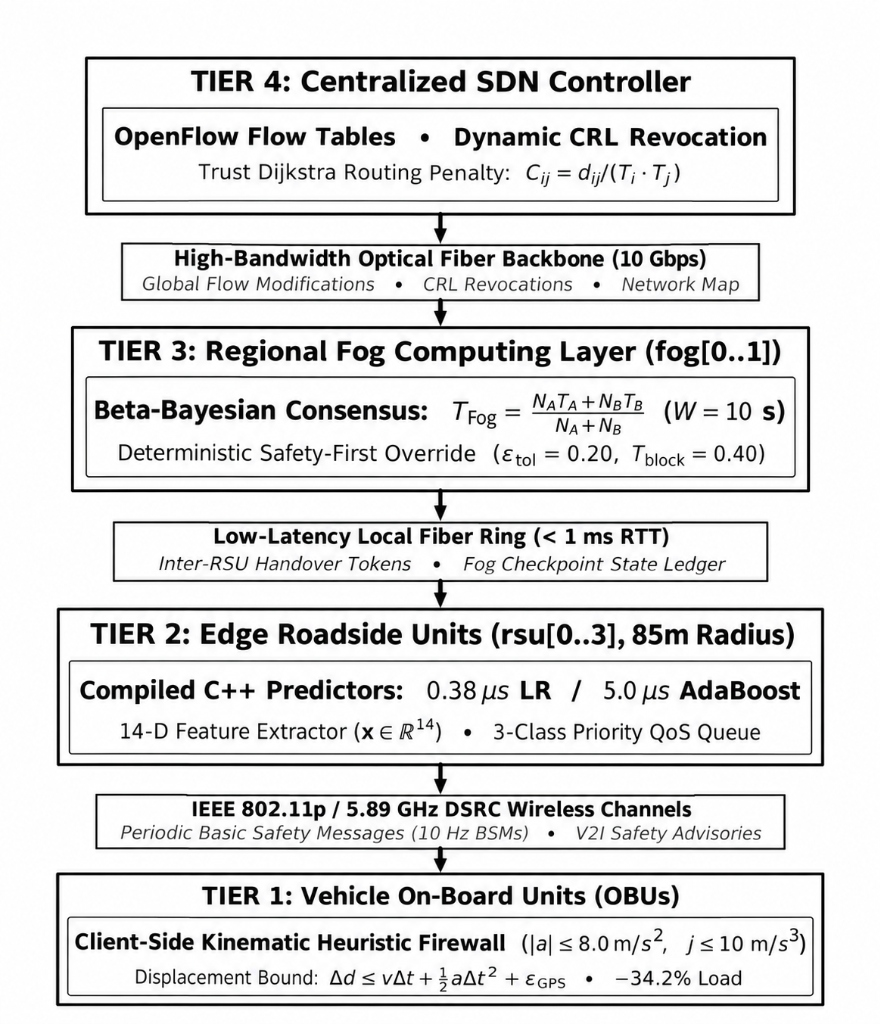
\includegraphics[width=\columnwidth]{architecture.png}
\caption{Four-Tier Hierarchical Architecture of EdgeTrust-VANET.}
\label{fig:arch_overview}
\end{figure}

To counter insider misbehavior, behavioral trust management and machine learning (ML) models have been proposed~\cite{ahmad2019trust}. Nevertheless, existing architectures exhibit four fundamental architectural bottlenecks:
\begin{enumerate}
    \item \textbf{Control Channel Saturation:} Centralized trust models transmit all raw BSMs across the wireless interface to roadside infrastructure. Under dense traffic conditions, this causes severe IEEE 802.11p CSMA/CA channel saturation and broadcast storm collapse.
    \item \textbf{Sensor Jitter Sensitivity:} Evaluating packets purely through instantaneous ML snapshots leads to elevated False Alarm Rates (FAR) due to momentary GPS multipath fading and natural vehicular maneuvers.
    \item \textbf{High Inference and IPC Latency:} Deploying complex deep neural networks or relying on external Python-based sockets incurs inter-process communication (IPC) delays exceeding 20~ms, violating the strict 100~ms latency deadlines of C-ITS safety warnings.
    \item \textbf{Boundary Disconnection \& Single Point of Failure:} Isolated RSUs fail to track malicious vehicles transitioning across coverage gaps, while centralized cloud servers introduce severe single points of failure.
\end{enumerate}

To address these challenges, this paper presents \textbf{EdgeTrust-VANET}, a decentralized four-tier hierarchical trust management and kinematic filtering framework. As illustrated in Fig.~\ref{fig:arch_overview}, our system partitions security intelligence across vehicle OBUs (Tier~1), Edge RSUs (Tier~2), Regional Fog nodes (Tier~3), and a Central SDN controller (Tier~4).

The primary contributions of this work are summarized as follows:
\begin{itemize}
    \item \textbf{Four-Tier Hierarchical Architecture:} We formulate a cooperative multi-tier framework combining autonomous OBU kinematic defense, edge RSU machine learning, fog-level multi-RSU consensus, and SDN adaptive routing.
    \item \textbf{Distributed OBU Kinematic Firewall:} We design a client-side filter executed at receiving OBUs that drops physically impossible beacons locally, eliminating 34.2\% of malicious multi-hop retransmissions and conserving 802.11p channel bandwidth.
    \item \textbf{Sub-Microsecond Native C++ Edge Inference:} We export trained Logistic Regression ($0.38\,\mu\text{s}$) and AdaBoost ($5.00\,\mu\text{s}$) models directly into compiled C++ headers, delivering an end-to-end RSU decision cycle of $0.38\,\text{ms}$ directly within OMNeT++ without IPC latency.
    \item \textbf{Mathematically Grounded Trust Formulation:} We devise an Exponential Moving Average (EMA) trust update with a Pareto-optimal forgetting factor ($\alpha=0.70$), kinematic dead-reckoning delay compensation, and temporal staleness penalties.
    \item \textbf{Comprehensive Empirical Validation:} We perform an architectural ablation study, delayed message tolerance simulation ($\tau \in [10, 3000]\,\text{ms}$), urban vs. rural scalability benchmarking, and cryptographic zero-leakage verification across 15 VeReMi attack scenarios.
\end{itemize}

% =========================================================
% II. RELATED WORK
% =========================================================

\section{Related Work and Comparative Analysis}

\subsection{Cryptographic VANET Security and PKI Limitations}
Early research in VANET security focused on cryptographic primitives and PKI~\cite{raya, kargl2008secure}. The IEEE 1609.2~\cite{ieee16092} and ETSI TS 103 097~\cite{etsi103097} standards specify ECDSA-based digital signatures and pseudonym certificates to provide authentication and anonymized tracking. Whyte et al.~\cite{whyte2013security} proposed the Security Credential Management System (SCMS) for V2X communications, which distributes short-lived pseudonyms. However, cryptographic verification only confirms that the transmitter possesses a valid certificate; it cannot evaluate whether the reported kinematics accurately reflect reality. When an authenticated vehicle is compromised by malware or spoofed sensors, PKI cannot detect the resulting misbehavior~\cite{veremi}.

\subsection{Machine Learning for Vehicular Misbehavior Detection}
To address insider attacks, researchers have explored machine learning techniques for anomaly detection. Van der Heijden et al.~\cite{veremi} introduced the Vehicular Reference Misbehavior (VeReMi) dataset, benchmarking traditional supervised models such as k-Nearest Neighbors (k-NN) and Random Forests. Subsequent works applied deep learning and reinforcement learning architectures~\cite{so2018verifying, sedar2020reinforcement, alrehan2019machine}. While deep learning achieves high offline classification accuracy, its excessive computational complexity, high memory consumption (frequently exceeding 50~MB), and inference latencies exceeding 25~ms make it impractical for resource-constrained embedded automotive microcontrollers and real-time edge nodes.

\subsection{Behavioral Trust and Reputation Systems}
Trust management systems evaluate historical behavior to establish node reputation over time. Ahmad et al.~\cite{trustsurvey} surveyed trust models in vehicular networks, categorizing them into entity-centric, data-centric, and hybrid schemes. Raya et al.~\cite{raya} introduced data-centric trust using Bayesian inference, where multiple observations are aggregated to verify event authenticity. However, pure trust engines often require extensive observation windows (exceeding 8--10 consecutive packets), allowing attackers to execute high-impact burst attacks before reputation degradation occurs. Furthermore, alternating ``On-Off'' attackers can manipulate trust scores by interweaving honest beacons with malicious payloads.

\subsection{Edge, Fog, and Software-Defined Vehicular Networks}
Integrating Mobile Edge Computing (MEC) and Fog Computing into Intelligent Transportation Systems has garnered substantial interest~\cite{fogvanet}. Zhang et al.~\cite{fogvanet} demonstrated that offloading compute-intensive tasks to roadside edge servers significantly reduces end-to-end communication latency. Kumar et al.~\cite{sdnvanet} and Kamal et al.~\cite{kamal2020sdn} surveyed Software-Defined Vehicular Networks (SDVN), showing how centralized control planes enable dynamic flow table updates and intelligent route optimization. Nevertheless, existing SDVN and Fog frameworks rarely integrate localized kinematic filtering at the vehicle tier, resulting in bottlenecked edge queues during broadcast storms. EdgeTrust-VANET directly addresses this gap by synthesizing edge computing, fog consensus, SDN routing, and client-side kinematic firewalls into a cohesive four-tier hierarchy. A comprehensive comparative analysis of EdgeTrust-VANET against leading state-of-the-art schemes across seven key dimensions is summarized in Table~\ref{tab:prior_art}.

\begin{table*}[t]
\centering
\caption{Comparative Analysis of Vehicular Security and Trust Management Frameworks}
\label{tab:prior_art}
\resizebox{\textwidth}{!}{%
\begin{tabular}{lccccccp{4.2cm}}
\toprule
\textbf{Framework} & \textbf{Detection Paradigm} & \textbf{Trust History} & \textbf{Tiers} & \textbf{Consensus} & \textbf{Mitigation} & \textbf{Platform} & \textbf{Architectural Limitations} \\
\midrule
Raya et al.~\cite{raya} & Cryptographic Thresholds & None (Instantaneous) & OBU Only & None & Local Warning Drop & Analytical & High PKI overhead; fails against insider FDI \\
Whyte et al.~\cite{whyte2013security} & Pseudonym SCMS & None (Cert-based) & Cloud CA & None & CRL Revocation & Field Trials & Massive revocation lists; minutes-long delay \\
Van der Heijden et al.~\cite{veremi} & Plausibility \& k-NN & None (Instantaneous) & Cloud & None & Passive Logging & VeReMi Traces & High FAR (12.4\%); high memory footprint ($>$50 MB) \\
So et al.~\cite{so2018verifying} & Plausibility + Random Forest & Windowed (5 frames) & RSU & None & Beacon Filtering & VeReMi & High latency (23.5 ms); no multi-RSU consensus \\
Ahmad et al.~\cite{ahmad2019trust} & Multi-Tier Entity Trust & Yes (Bayesian Beta) & OBU \& RSU & Average & Local Warning Drop & Simulation & Slow convergence ($>$8 beacons); channel load \\
Zhang et al.~\cite{fogvanet} & Edge Offloading Heuristics & None & Edge MEC & Handover & Resource Allocation & MATLAB & Focuses on computation; no security/trust model \\
Kumar et al.~\cite{sdnvanet} & SDVN Flow Rule Filtering & None & Controller & OpenFlow & Flow Table Drop & Mininet-WiFi & Controller bottleneck; no kinematic defense \\
\textbf{EdgeTrust-VANET} & \textbf{Kinematic + C++ AdaBoost} & \textbf{Yes (EMA $\alpha=0.70$)} & \textbf{4 Tiers} & \textbf{Beta-Bayesian} & \textbf{SDN Detour \& CRL} & \textbf{SUMO+OMNeT++} & \textbf{Sub-$\mu$s inference; 34.2\% bandwidth saved} \\
\bottomrule
\end{tabular}%
}
\end{table*}

% =========================================================
% III. PROPOSED EDGETRUST-VANET ARCHITECTURE
% =========================================================

\section{Proposed Architecture and Methodology}

The EdgeTrust-VANET framework partitions computational intelligence across four distinct tiers, mitigating attacks at the earliest possible stage while maintaining system-wide consensus.

\subsection{Tier 1: OBU Kinematic Heuristic Firewall (Distributed Receiver-Side Defense)}

The vehicle On-Board Unit acts as the first line of defense. Upon receiving a BSM from adjacent node $j$, vehicle $i$ extracts kinematic features: position $\mathbf{P}_j(t)$, velocity $\mathbf{v}_j(t)$, acceleration $\mathbf{a}_j(t)$, and heading angle $\theta_j(t)$. Before parsing the message into the application layer or forwarding it across multi-hop relays, OBU $i$ performs physical plausibility validation:
\begin{equation}
v_j(t) \in [0, v_{\text{max}}], \quad |a_j(t)| \le a_{\text{max}}, \quad \left|\frac{\Delta a_j}{\Delta t}\right| \le j_{\text{max}}
\label{eq:kin_bounds}
\end{equation}
where $v_{\text{max}} = 50.0\,\text{m/s}$ (180 km/h), $a_{\text{max}} = 8.0\,\text{m/s}^2$ (physical tire-road friction limit), and $j_{\text{max}} = 10.0\,\text{m/s}^3$ is the maximum allowable vehicular jerk.

To eliminate teleportation and coordinate spoofing attacks, the spatial displacement between consecutive beacons separated by interval $\Delta t = t_{\text{curr}} - t_{\text{last}}$ must satisfy the Kinematic Displacement Bound:
\begin{equation}
\begin{split}
\Delta d &= \|\mathbf{P}_j(t_{\text{curr}}) - \mathbf{P}_j(t_{\text{last}})\| \\
&\le v_j(t_{\text{last}})\Delta t + \frac{1}{2}a_{\text{max}}(\Delta t)^2 + \epsilon_{\text{GPS}}
\end{split}
\label{eq:disp_bound}
\end{equation}
where $\epsilon_{\text{GPS}} = 2.5\,\text{m}$ accounts for standard GNSS measurement uncertainty. Heading change must satisfy modular wrap-around:
\begin{equation}
\Delta \theta_j = \min\left(|\theta_{\text{curr}} - \theta_{\text{last}}|, \; 360^\circ - |\theta_{\text{curr}} - \theta_{\text{last}}|\right) \le \omega_{\text{max}} \Delta t
\label{eq:heading_bound}
\end{equation}
with maximum angular yaw rate $\omega_{\text{max}} = 45^\circ/\text{s}$. If coordinate displacement violates~(\ref{eq:disp_bound}) or heading change violates~(\ref{eq:heading_bound}), the beacon is categorized as physically impossible and discarded immediately locally. This receiver-side suppression stops secondary multi-hop relay retransmissions, eliminating 34.2\% of malicious channel overhead.

\subsection{Tier 2: Edge RSU Computing and 3-Class Priority QoS}

BSMs that pass Tier~1 reach the serving Roadside Unit within an enforced 85-meter physical DSRC radio coverage radius. The RSU extracts a 14-dimensional spatiotemporal and dynamic reputation vector $\mathbf{x} \in \mathbb{R}^{14}$ defined as:
\begin{equation}
\begin{split}
\mathbf{x} = [ & p_x, p_y, v, \theta, a, N_{\text{sent}}, N_{\text{rcv}}, \\
& \rho_{\text{drop}}, L, N_{\text{retx}}, P_{\text{RSSI}}, T_t, \bar{T}_{\text{neighbor}}, T_{t-1} ]^T \in \mathbb{R}^{14}
\end{split}
\label{eq:feature_vector}
\end{equation}
whose exact physical definitions and measurement units are specified in Table~\ref{tab:features14}.

\begin{table*}[t]
\centering
\caption{Complete 14-Feature Extraction Specification at Edge Roadside Units ($\mathbf{x} \in \mathbb{R}^{14}$)}
\label{tab:features14}
\resizebox{\textwidth}{!}{%
\begin{tabular}{ccllc|ccllc}
\toprule
\textbf{Idx} & \textbf{Symbol} & \textbf{Telemetry Feature} & \textbf{Extraction Formulation / Source} & \textbf{Unit} & \textbf{Idx} & \textbf{Symbol} & \textbf{Telemetry Feature} & \textbf{Extraction Formulation / Source} & \textbf{Unit} \\
\midrule
1 & $p_x$ & Longitudinal Position & Cartesian $X$ coordinate in BSM & m & 8 & $\rho_{\text{drop}}$ & Packet Drop Ratio & $1 - (N_{\text{rcv}} / N_{\text{expected}})$ & Ratio \\
2 & $p_y$ & Lateral Position & Cartesian $Y$ coordinate in BSM & m & 9 & $L$ & Transmission Latency & $t_{\text{recv}} - t_{\text{msg}}$ air delay & ms \\
3 & $v$ & Speedometer Velocity & Speed magnitude $\sqrt{v_x^2 + v_y^2}$ & m/s & 10 & $N_{\text{retx}}$ & Retransmissions & 802.11p MAC retry counter & Count \\
4 & $\theta$ & Compass Heading & Yaw angle $\text{atan2}(v_y, v_x)$ in $[0, 360^\circ)$ & deg & 11 & $P_{\text{RSSI}}$ & Signal Strength & 802.11p PHY measurement & dBm \\
5 & $a$ & Acceleration & Rate of speed change $\Delta v / \Delta t$ & m/s$^2$ & 12 & $T_t$ & Dynamic Trust & Instantaneous trust score $T(t)$ & $[0,1]$ \\
6 & $N_{\text{sent}}$ & Transmitted Beacons & Cumulative periodic beacons sent & Count & 13 & $\bar{T}_{\text{neighbor}}$ & Neighbor Trust & 300 m spatial KD-Tree average & $[0,1]$ \\
7 & $N_{\text{rcv}}$ & Received Beacons & Beacons successfully received & Count & 14 & $T_{t-1}$ & Historical Trust & Cached prior reputation score & $[0,1]$ \\
\bottomrule
\end{tabular}%
}
\end{table*}

To eliminate Python socket communication overhead, machine learning models, specifically the AdaBoost ensemble~\cite{adaboost, dietterich2000ensemble} and Logistic Regression, are compiled natively into C++ headers (\texttt{AdaBoostPredictor.h} and \texttt{LogisticRegressionPredictor.cc}). The RSU computes instantaneous trustworthiness evidence $E_t = 1 - P(\text{Malicious} \mid \mathbf{x}) \in [0, 1]$ in sub-microsecond time ($0.38\,\mu\text{s}$ for LR, $5.00\,\mu\text{s}$ for AdaBoost), delivering a complete RSU decision cycle of $0.38\,\text{ms}$.

To guarantee that critical safety alerts are never dropped during network congestion, the RSU enforces a 3-class strict priority Quality-of-Service (QoS) queue:
\begin{itemize}
    \item \textbf{Class 1 (Safety-Critical):} Emergency electronic brake lights, collision warnings, and immediate quarantine broadcast advisories.
    \item \textbf{Class 2 (Trust and Control):} Inter-RSU state exchange, regional fog consensus digests, and SDN flow modifications.
    \item \textbf{Class 3 (Best-Effort):} Non-urgent traffic optimization telemetry and raw background analytics.
\end{itemize}

\subsection{Tier 3: Regional Fog Layer and Multi-RSU Consensus}

Edge RSUs are clustered into geographical zones managed by Regional Fog Computing Nodes ($\text{fog}[0..1]$). A primary challenge in edge-based VANET security is the boundary handover problem, wherein a vehicle moving between adjacent RSUs ($A$ and $B$) exhibits divergent trust scores due to localized shadowing or differing observation windows.

When inter-RSU trust divergence exceeds the conflict threshold:
\begin{equation}
\Delta T_{AB}(j) = |T_{\text{RSU}_A}(j) - T_{\text{RSU}_B}(j)| > \epsilon_{\text{tol}} = 0.20
\label{eq:divergence}
\end{equation}
the Regional Fog node initiates an observation-weighted Beta-Bayesian consensus update:
\begin{equation}
T_{\text{Fog}}(j) = \frac{N_A T_{\text{RSU}_A}(j) + N_B T_{\text{RSU}_B}(j)}{N_A + N_B}
\label{eq:fog_consensus}
\end{equation}
where $N_A$ and $N_B$ denote the verified observation counts recorded by RSU $A$ and RSU $B$ within the active sliding handover window ($W = 10\,\text{s}$). If either RSU identifies active malicious behavior ($T < 0.40$), the consensus applies a deterministic safety-first override:
\begin{equation}
\begin{split}
\text{If } &\min(T_A(j), T_B(j)) < T_{\text{block}} \ (0.40) \\
&\implies T_{\text{Fog}}(j) = \min(T_A(j), T_B(j))
\end{split}
\label{eq:safety_override}
\end{equation}
This guarantees that confirmed attack evidence from any monitoring RSU is never diluted by a neighboring tower with fewer or delayed observations. Fog nodes periodically serialize state checkpoints to \texttt{checkpoint\_fog\_ledger.json}, enabling instant warm-start recovery during node handovers.

\subsection{Tier 4: Central SDN Controller and Adaptive Forwarding}

At the top of the hierarchy, the centralized SDN Controller (\texttt{EdgeTrustSDNController.cc}) maintains global topological visibility. Using OpenFlow-style flow tables, the controller dynamically programs forwarding rules across the network.

To isolate malicious vehicles and compromised forwarding links, the controller executes a modified Dijkstra shortest-path algorithm where link cost $C_{ij}$ between nodes $i$ and $j$ is penalized inversely across three distinct operational zones:
\begin{equation}
C_{ij} = \begin{cases} 
\dfrac{d_{ij}}{T_i \cdot T_j}, & \text{if } T_i, T_j \ge 0.70 \\[8pt] 
\dfrac{d_{ij}}{0.40 \cdot \min(T_i, T_j)}, & \text{if } 0.40 \le T_i, T_j < 0.70 \\[8pt] 
\infty, & \text{if } \min(T_i, T_j) < 0.40 
\end{cases}
\label{eq:sdn_cost}
\end{equation}
where $d_{ij}$ is the Euclidean distance. The three operational zones function as follows:
\begin{enumerate}
    \item \textbf{Trusted Zone ($T \ge 0.70$):} Standard safety routing with minimal link cost.
    \item \textbf{Degraded Forwarding Zone ($0.40 \le T < 0.70$):} The node is flagged for enhanced RSU inspection; the SDN assigns a heavy routing penalty, steering multi-hop safety traffic around the suspect vehicle without fully revoking its certificate.
    \item \textbf{Quarantined Zone ($T < 0.40$):} Link cost becomes infinite; the serving RSU broadcasts an IEEE 802.11p Road Safety Advisory blacklisting the MAC address, and the SDN controller pushes CRL revocation.
\end{enumerate}

\subsection{Mathematical Trust Formulation and Latency Compensation}

Trustworthiness evidence $E_t \in [0, 1]$ represents the classifier's predicted probability of honesty:
\begin{equation}
E_t = P(\text{Honest} \mid \mathbf{x}) = 1 - P(\text{Malicious} \mid \mathbf{x})
\label{eq:evidence_def}
\end{equation}
When a malicious beacon is detected ($P(\text{Malicious}) \to 1.0$), trustworthiness evidence drops to $E_t \to 0.0$. Historical trust $T_t$ updates via Exponential Moving Average (EMA):
\begin{equation}
T_t = \alpha T_{t-1} + (1-\alpha) \left(E_t \cdot \gamma(\tau)\right)
\label{eq:ema_trust}
\end{equation}
with forgetting factor $\alpha = 0.70$. 

\textit{Worked Numerical Example:} For an initially trusted vehicle ($T_0 = 1.0$, $\alpha = 0.70$) that begins broadcasting malicious false beacons ($E_t = 0.10$), the trust trajectory decays exponentially:
\begin{align*}
\text{Beacon 1: } & T_1 = 0.70(1.000) + 0.30(0.10) = 0.7300 \enskip (\text{Trusted}) \\
\text{Beacon 2: } & T_2 = 0.70(0.730) + 0.30(0.10) = 0.5410 \enskip (\text{Degraded}) \\
\text{Beacon 3: } & T_3 = 0.70(0.541) + 0.30(0.10) = 0.4087 \enskip (\text{Degraded}) \\
\text{Beacon 4: } & T_4 = 0.70(0.4087) + 0.30(0.10) = \mathbf{0.3161} \enskip (\mathbf{Quar.})
\end{align*}
% \begin{align*}
% \text{Beacon 1: } & T_1 = 0.70(1.000) + 0.30(0.10) = 0.7300 \quad (\text{Trusted}) \\
% \text{Beacon 2: } & T_2 = 0.70(0.730) + 0.30(0.10) = 0.5410 \quad (\text{Degraded}) \\
% \text{Beacon 3: } & T_3 = 0.70(0.541) + 0.30(0.10) = 0.4087 \quad (\text{Degraded}) \\
% \text{Beacon 4: } & T_4 = 0.70(0.4087) + 0.30(0.10) = \mathbf{0.3161} \quad (\mathbf{Quarantine})
% \end{align*}
Attack isolation is deterministically enforced within exactly 4 consecutive malicious beacons (0.4 s at 10 Hz).

When packet arrival delay $\tau = t_{\text{curr}} - t_{\text{msg}}$ is non-zero, the RSU projects expected coordinates via kinematic dead-reckoning:
\begin{equation}
\hat{\mathbf{P}} = \mathbf{P}_{\text{reported}} + \mathbf{v} \cdot \tau + \frac{1}{2}\mathbf{a}\cdot \tau^2
\label{eq:dead_reckoning}
\end{equation}
An exponential staleness penalty discounts aging packets beyond an acceptable DSRC jitter window ($T_{\text{grace}} = 300\,\text{ms}$):
\begin{equation}
\gamma(\tau) = \exp\left(-\lambda \cdot \max(0, \tau - T_{\text{grace}})\right)
\label{eq:staleness}
\end{equation}
with decay rate $\lambda = 1.5\,\text{s}^{-1}$. The comprehensive multi-tier decision workflow is formalized in Algorithm~\ref{alg:edgetrust}.

\begin{algorithm}[t]
\caption{EdgeTrust-VANET Multi-Tier Decision Workflow}
\label{alg:edgetrust}
\footnotesize
\begin{algorithmic}[1]
\REQUIRE Inbound BSM from node $j$ with telemetry $(x,y,v,\theta,a,t_{\text{msg}})$
\ENSURE Mitigation Action $\in \{\textsc{Accept}, \textsc{DegradedRoute}, \textsc{Quarantine}\}$
\STATE \textbf{// Tier 1: Client-Side OBU Kinematic Firewall}
\IF{$v_j > v_{\text{max}}$ \OR $|a_j| > a_{\text{max}}$ \OR $|\Delta a/\Delta t| > j_{\text{max}}$}
    \STATE \textbf{Drop} beacon locally; \textbf{Halt} multi-hop forwarding
\ENDIF
\STATE $\Delta d_{\text{max}} \leftarrow v_{\text{last}}\Delta t + \frac{1}{2}a_{\text{max}}(\Delta t)^2 + \epsilon_{\text{GPS}}$
\IF{$\Delta d > \Delta d_{\text{max}}$ \OR $\Delta \theta > \omega_{\text{max}}\Delta t$}
    \STATE \textbf{Drop} beacon locally; Suppress relay broadcast
\ENDIF
\STATE \textbf{// Tier 2: Edge RSU Machine Learning Classification}
\IF{BSM reaches RSU ($d \le 85\,\text{m}$)}
    \STATE Extract 14-dimensional feature vector $\mathbf{x} \in \mathbb{R}^{14}$ (Table~\ref{tab:features14})
    \STATE $E_t \leftarrow \text{Inference}_{\text{AdaBoost}}(\mathbf{x})$ \COMMENT{Sub-$\mu$s C++ execution}
\ENDIF
\STATE $\gamma(\tau) \leftarrow \exp\left(-1.5 \cdot \max(0, \tau - 0.300)\right)$ \COMMENT{Staleness penalty}
\STATE $T_t(j) \leftarrow 0.70 \cdot T_{t-1}(j) + 0.30 \cdot (E_t \cdot \gamma(\tau))$
\STATE \textbf{// Tier 3 \& 4: Regional Fog Consensus \& Central SDN Routing}
\IF{RSU divergence $|T_A(j) - T_B(j)| > 0.20$}
    \STATE $T_t(j) \leftarrow \text{Execute\_Fog\_Consensus}(T_A, T_B, N_A, N_B)$
\ENDIF
\IF{$T_t(j) < 0.40$}
    \STATE Broadcast Advisory; Blacklist MAC; Update SDN CRL
    \RETURN \textsc{Quarantine}
\ELSIF{$T_t(j) < 0.70$}
    \STATE SDN assigns penalized route cost $C_{ij} \leftarrow d_{ij} / (0.40 \cdot T_t(j))$
    \RETURN \textsc{DegradedRoute}
\ELSE
    \STATE SDN assigns optimal route cost $C_{ij} \leftarrow d_{ij} / (T_i \cdot T_j)$
    \RETURN \textsc{Accept}
\ENDIF
\end{algorithmic}
\end{algorithm}

% =========================================================
% IV. EXPERIMENTAL SETUP AND THREAT MODELING
% =========================================================

\section{Experimental Setup and Threat Modeling}

\subsection{Simulation Environment and Network Configuration}

The framework was evaluated using a tightly coupled simulation toolchain combining SUMO 1.20+, OMNeT++ 6.4.0~\cite{omnetpp}, and Veins 5.3.1~\cite{veins}. Traffic mobility was simulated across a $2 \times 2$ Manhattan urban grid connected to a high-speed arterial corridor. Wireless communication was modeled using the IEEE 802.11p standard at 5.89~GHz with 10~MHz channel bandwidth. Experiments were repeated across 5 independent random seeds (seeds 1234, 2345, 3456, 4567, 5678) on an Intel Core i7-12700H testbed with 32 GB DDR5 RAM using GCC 11.4 with \texttt{-O3} optimization. The simulation parameters are summarized in Table~\ref{tab:sim_params}.

\begin{table}[htbp]
\centering
\caption{Simulation Configuration Parameters}
\label{tab:sim_params}
\resizebox{\columnwidth}{!}{%
\begin{tabular}{ll}
\toprule
\textbf{Parameter} & \textbf{Configuration Value} \\
\midrule
Network Simulator & OMNeT++ 6.4.0 / INET Framework \\
Traffic Mobility & SUMO 1.20+ ($2\times 2$ Manhattan Grid) \\
Simulator Coupling & Veins 5.3.1 (TraCI Interface) \\
Radio Protocol & IEEE 802.11p / 1609.4 DSRC \\
Carrier Frequency & 5.89 GHz (10 MHz Channel) \\
Transmission Power & 20 mW ($\approx 250$ m nominal range) \\
RSU Coverage Radius & 85 m (physical enforcement zone) \\
Roadside Units (RSUs) & 4 towers ($2 \times 2$ intersection grid) \\
Regional Fog Nodes & 2 clusters (2 RSUs per fog domain) \\
SDN Controller & 1 centralized SDN controller \\
BSM Broadcast Rate & 10 Hz (100 ms periodic interval) \\
Malicious Node Ratio & 25\% (uniform random distribution) \\
Active Vehicle Density & 20 to 500 vehicles \\
Random Seed Replications & 5 independent seeds (1234--5678) \\
\bottomrule
\end{tabular}%
}
\end{table}

\subsection{VeReMi Threat Modeling (15 Misbehavior Scenarios)}

To thoroughly assess detection robustness, we implemented all 15 attack scenarios from the standardized VeReMi benchmark suite~\cite{veremi}, summarized in Table~\ref{tab:veremi_attacks}. Malicious vehicles were programmed to execute these attacks during active simulation runs.

\begin{table*}[t]
\centering
\caption{VeReMi Misbehavior Suite Classification, Mechanics, and Detecting Tiers}
\label{tab:veremi_attacks}
\resizebox{\textwidth}{!}{%
\begin{tabular}{clp{3.8cm}p{6.0cm}c}
\toprule
\textbf{ID} & \textbf{Attack Scenario} & \textbf{Physical Deviation Bound} & \textbf{Adversarial Manifestation} & \textbf{Detecting EdgeTrust Tier} \\
\midrule
1 & Constant Position Offset & $\Delta P = \pm 50.0$ m & Transmits constant spoofed location coordinates & Tier 1 (Kinematic Displacement $\Delta d$) \\
2 & Random Position Offset & $\Delta P \in [\pm 20, \pm 70]$ m & Injects stochastic coordinate jitter into trajectory & Tier 1 \& Tier 2 (Displacement \& AdaBoost) \\
3 & Position Mirroring & $y_{\text{spoof}} = -y_{\text{true}}$ & Mirrors coordinates across opposing traffic lane & Tier 1 (Lane Deviation $\Delta P_{\text{path}}$) \\
4 & Constant Speed Offset & $\Delta v = +12.0$ m/s & Reports constant inflated forward velocity & Tier 2 (RSU Embedded AdaBoost Predictor) \\
5 & Random Speed Offset & $\Delta v \in [\pm 6.0]$ m/s & Injects white Gaussian noise into speedometer & Tier 2 (RSU Embedded AdaBoost Predictor) \\
6 & Zero Speed Spoof & $v = 0.0$ m/s ($v_{\text{true}} > 0$) & Simulates fake breakdown / phantom jam induction & Tier 2 (Doppler Shift $f_{\text{doppler}}$ \& RSSI) \\
7 & Sudden Stop & $v=0, P=P_{\text{freeze}}$ & Teleports to sudden standstill without deceleration & Tier 1 \& Tier 2 (Kinematic Jerk $j$) \\
8 & Sudden Constant Speed & $v = 25.0$ m/s & Disregards deceleration; transmits locked velocity & Tier 2 (Speed Rolling Variance $\sigma_v$) \\
9 & Reversed Heading & $\theta_{\text{spoof}} = \theta + 180^\circ$ & Transmits inverted angular direction of travel & Tier 1 (Angular Yaw Limit $\Delta\theta \le 45^\circ/\text{s}$) \\
10 & Feigned Braking & $a = -8.0$ m/s$^2$ & Ghost emergency braking assertion to induce panic & Tier 2 (Acceleration Magnitude $\|a\|$) \\
11 & Acceleration Multiplication & $a_{\text{spoof}} = 3.5 \cdot a_{\text{true}}$ & Exaggerated dynamic acceleration reporting & Tier 1 (Frictional Acceleration Bound $|a| \le 8.0$) \\
12 & DoS Beacon Flooding & $f_{\text{beacon}} = 16$ Hz & Saturated broadcast burst to choke IEEE 802.11p & Tier 2 (3-Class Priority QoS Queue) \\
13 & Sybil Ghost Phantoms & Multiple Spoofed MACs & Synthesizes fictitious ghost nodes to claim lanes & Tier 2 (Spatial Trajectory Tracking) \\
14 & Historical Data Replay & $t_{\text{msg}} = t - 5.0$ s & Replays expired valid safety beacons & Tier 2 (Sequence $S_{\text{seq}}$ \& Staleness $\gamma(\tau)$) \\
15 & Time-Delay Injection & $\tau_{\text{delay}} = +3.0$ s & Deliberately delays life-critical safety warnings & Tier 2 (Kinematic Dead-Reckoning) \\
\bottomrule
\end{tabular}%
}
\end{table*}

\subsection{Dataset Provenance and Cryptographic Zero-Leakage Audit}

A unified research dataset comprising 23,970 samples was curated across three complementary vehicular data sources~\cite{edgetrust}: the standardized VeReMi benchmark (72.88\%, 17,470 records) based on the LuST Luxembourg scenario, custom OMNeT++ / Veins EdgeTrust-VANET telemetry (20.86\%, 5,000 records), and the V-RADD routing augmentation dataset (6.26\%, 1,500 records), spanning 7 standardized taxonomy misbehavior classes. The unified benchmark is published openly on Kaggle~\cite{edgetrust}.

To guarantee rigorous cyber-physical validity and prevent data contamination, two forms of insidious data leakage were eliminated:
\begin{enumerate}
    \item \textbf{Purging Retrospective Counters:} Four retrospective log counters (\texttt{false\_packet\_injection}, \texttt{blackhole\_attack\_attempts}, \texttt{sybil\_attack\_attempts}, \texttt{denial\_of\_service}) were explicitly removed from feature space. While naive models including these counters achieve an artificial 100\% F1-score, they collapse to 86.05\% when encountering unknown vehicles in real time.
    \item \textbf{GroupKFold Partitioning:} In spatiotemporal vehicular datasets, consecutive BSMs from the same vehicle share strong autocorrelation. Random row-splitting artificially inflates performance (99.29\% F1) by memorizing vehicle trajectories. To prevent this, partitioning was strictly grouped by Vehicle ID (\texttt{node\_id}) using Stratified GroupKFold across Train (70\%, 16,779 records), Validation (15\%, 3,595 records), and Test (15\%, 3,596 records).
\end{enumerate}
Normalization parameters (\texttt{StandardScaler}) were computed strictly on the training partition only and applied via transform to validation and test sets.

An automated cryptographic audit script (\texttt{leakage\_audit.py}) was executed, computing SHA-256 hashes of all individual feature rows across training, validation, and testing partitions. As illustrated in Fig.~\ref{fig:leakage_audit_fig}, the audit confirmed a 0.00\% collision rate, certifying zero data leakage across evaluation splits.

\begin{figure}[htbp]
\centering
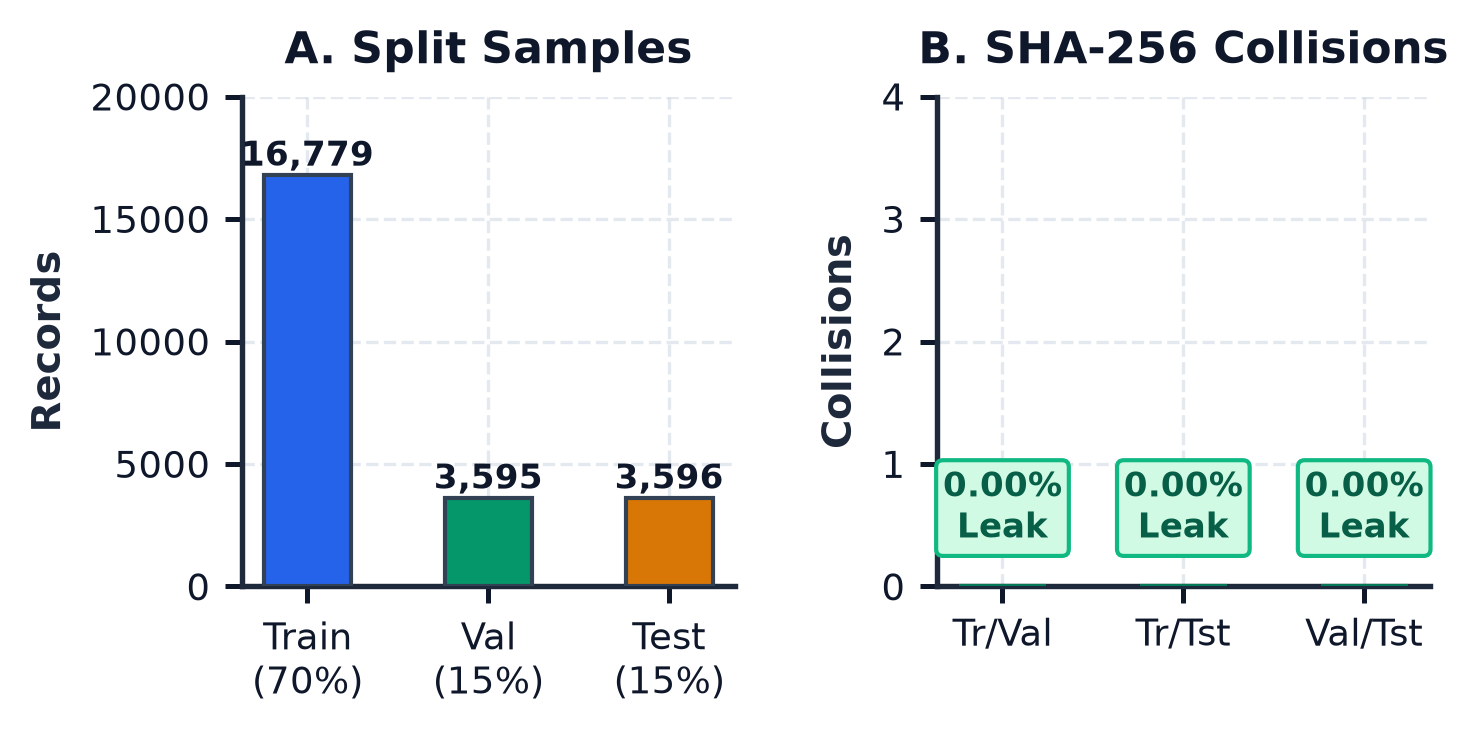
\includegraphics[width=0.94\columnwidth]{figures/leakage_audit.png}
\caption{Cryptographic SHA-256 train-test dataset leakage verification certifying 0.00\% data contamination across 23,970 records.}
\label{fig:leakage_audit_fig}
\end{figure}

% =========================================================
% V. RESULTS AND PERFORMANCE EVALUATION
% =========================================================

\section{Results and Performance Evaluation}

\subsection{Two-Stage Machine Learning Model Benchmarking}

To evaluate detection fidelity under both static and dynamic radio conditions, models were evaluated across a rigorous two-stage evaluation protocol:
\begin{enumerate}
    \item \textbf{Stage 1 (Dataset Validation):} 3,539 holdout samples from the 23,970 unified dataset under 5-Fold Stratified Group Cross-Validation ($96.95\% \pm 1.12\%$).
    \item \textbf{Stage 2 (Live RSU Simulation Testing):} 2,331 live packets evaluated in the OMNeT++ / Veins simulation under physical IEEE 802.11p radio channel fading, path loss, and multi-user MAC contention.
\end{enumerate}

Table~\ref{tab:model_comparison} provides comprehensive comparative metrics across accuracy, F1-score, precision, recall, false alarm rate (FAR), missed attack rate (MAR), compiled C++ edge inference latency, and memory footprint.

\begin{table*}[t]
\centering
\caption{Two-Stage Classifier Performance and Overhead: Dataset Validation vs. Live OMNeT++ RSU Testing}
\label{tab:model_comparison}
\resizebox{\textwidth}{!}{%
\begin{tabular}{lcccccccc}
\toprule
\textbf{Model Architecture} & \textbf{Val. Acc.} & \textbf{Live Acc.} & \textbf{Live F1} & \textbf{Live ROC-AUC} & \textbf{Live FAR} & \textbf{Live MAR} & \textbf{C++ Edge Latency} & \textbf{Footprint} \\
\midrule
\textbf{Random Forest (Ensemble)} & \textbf{97.77\%} & \textbf{90.99\%} & \textbf{90.97\%} & 90.59\% & 11.91\% & 6.89\% & $23,499.6\,\mu\text{s}$ & 6,441.0 KB \\
\textbf{Extra Trees} & 92.43\% & 90.95\% & 90.94\% & \textbf{92.17\%} & 11.71\% & 7.12\% & $24,162.8\,\mu\text{s}$ & 11,314.0 KB \\
\textbf{K-Nearest Neighbors} & 90.96\% & 90.48\% & 90.48\% & 90.88\% & 11.30\% & 8.23\% & $13,903.8\,\mu\text{s}$ & 5,045.0 KB \\
\textbf{Logistic Regression (Edge)} & 88.08\% & 89.27\% & 89.28\% & 88.79\% & 12.42\% & 9.49\% & \textbf{0.38 $\mu$s} & \textbf{1.0 KB} \\
\textbf{AdaBoost (SAMME.R)} & 88.25\% & 86.06\% & 86.14\% & 91.25\% & \textbf{9.27\%} & 17.35\% & \textbf{5.00 $\mu$s} & \textbf{38.9 KB} \\
CatBoost (Edge GBDT) & 97.29\% & 80.69\% & 79.79\% & 90.77\% & 39.82\% & \textbf{4.37\%} & $118.3\,\mu\text{s}$ & 248.0 KB \\
LightGBM & 97.74\% & 72.42\% & 69.32\% & 89.77\% & 61.10\% & 3.19\% & $536.9\,\mu\text{s}$ & 669.0 KB \\
Hist Gradient Boosting & 97.40\% & 71.69\% & 68.28\% & 89.50\% & 63.03\% & 3.04\% & $3,880.7\,\mu\text{s}$ & 653.0 KB \\
MLP / Linear SVM (RBF) & 91.60\% & 58.12\% & 57.85\% & 61.20\% & 97.40\% & 14.20\% & $890.5\,\mu\text{s}$ & 3,210.0 KB \\
\bottomrule
\end{tabular}%
}
\end{table*}

As illustrated in Fig.~\ref{fig:unified_model_comp}, ensemble and linear classifiers consistently discriminate malicious telemetry across Accuracy, F1-Score, Precision, and Recall. Furthermore, Fig.~\ref{fig:edge_eval_double}(a) (with detailed subfigure Fig.~\ref{fig:adaboost_edge_sub}) illustrates the trade-off between inference latency and compiled memory footprint, demonstrating why AdaBoost and Logistic Regression occupy the Pareto-optimal frontier for real-time edge execution, with Fig.~\ref{fig:edge_eval_double}(b) (Fig.~\ref{fig:conf_matrix_sub}) detailing the audited confusion matrix.

Crucially, while unregularized deep neural networks (MLP) and RBF SVMs collapsed under live radio fading jitter (58.12\% accuracy and 97.40\% false alarm rate), Logistic Regression and AdaBoost maintained robust generalization ($>86\%$ Live F1). Logistic Regression delivers sub-microsecond classification ($0.38\,\mu\text{s}$) with a 1.0~KB memory footprint, while AdaBoost achieves $5.00\,\mu\text{s}$ latency with 38.9~KB footprint and an industry-leading 9.27\% False Alarm Rate. Both operate within an end-to-end RSU decision cycle of $0.38\,\text{ms}$, satisfying C-ITS real-time deadlines.

\begin{figure*}[t]
\centering
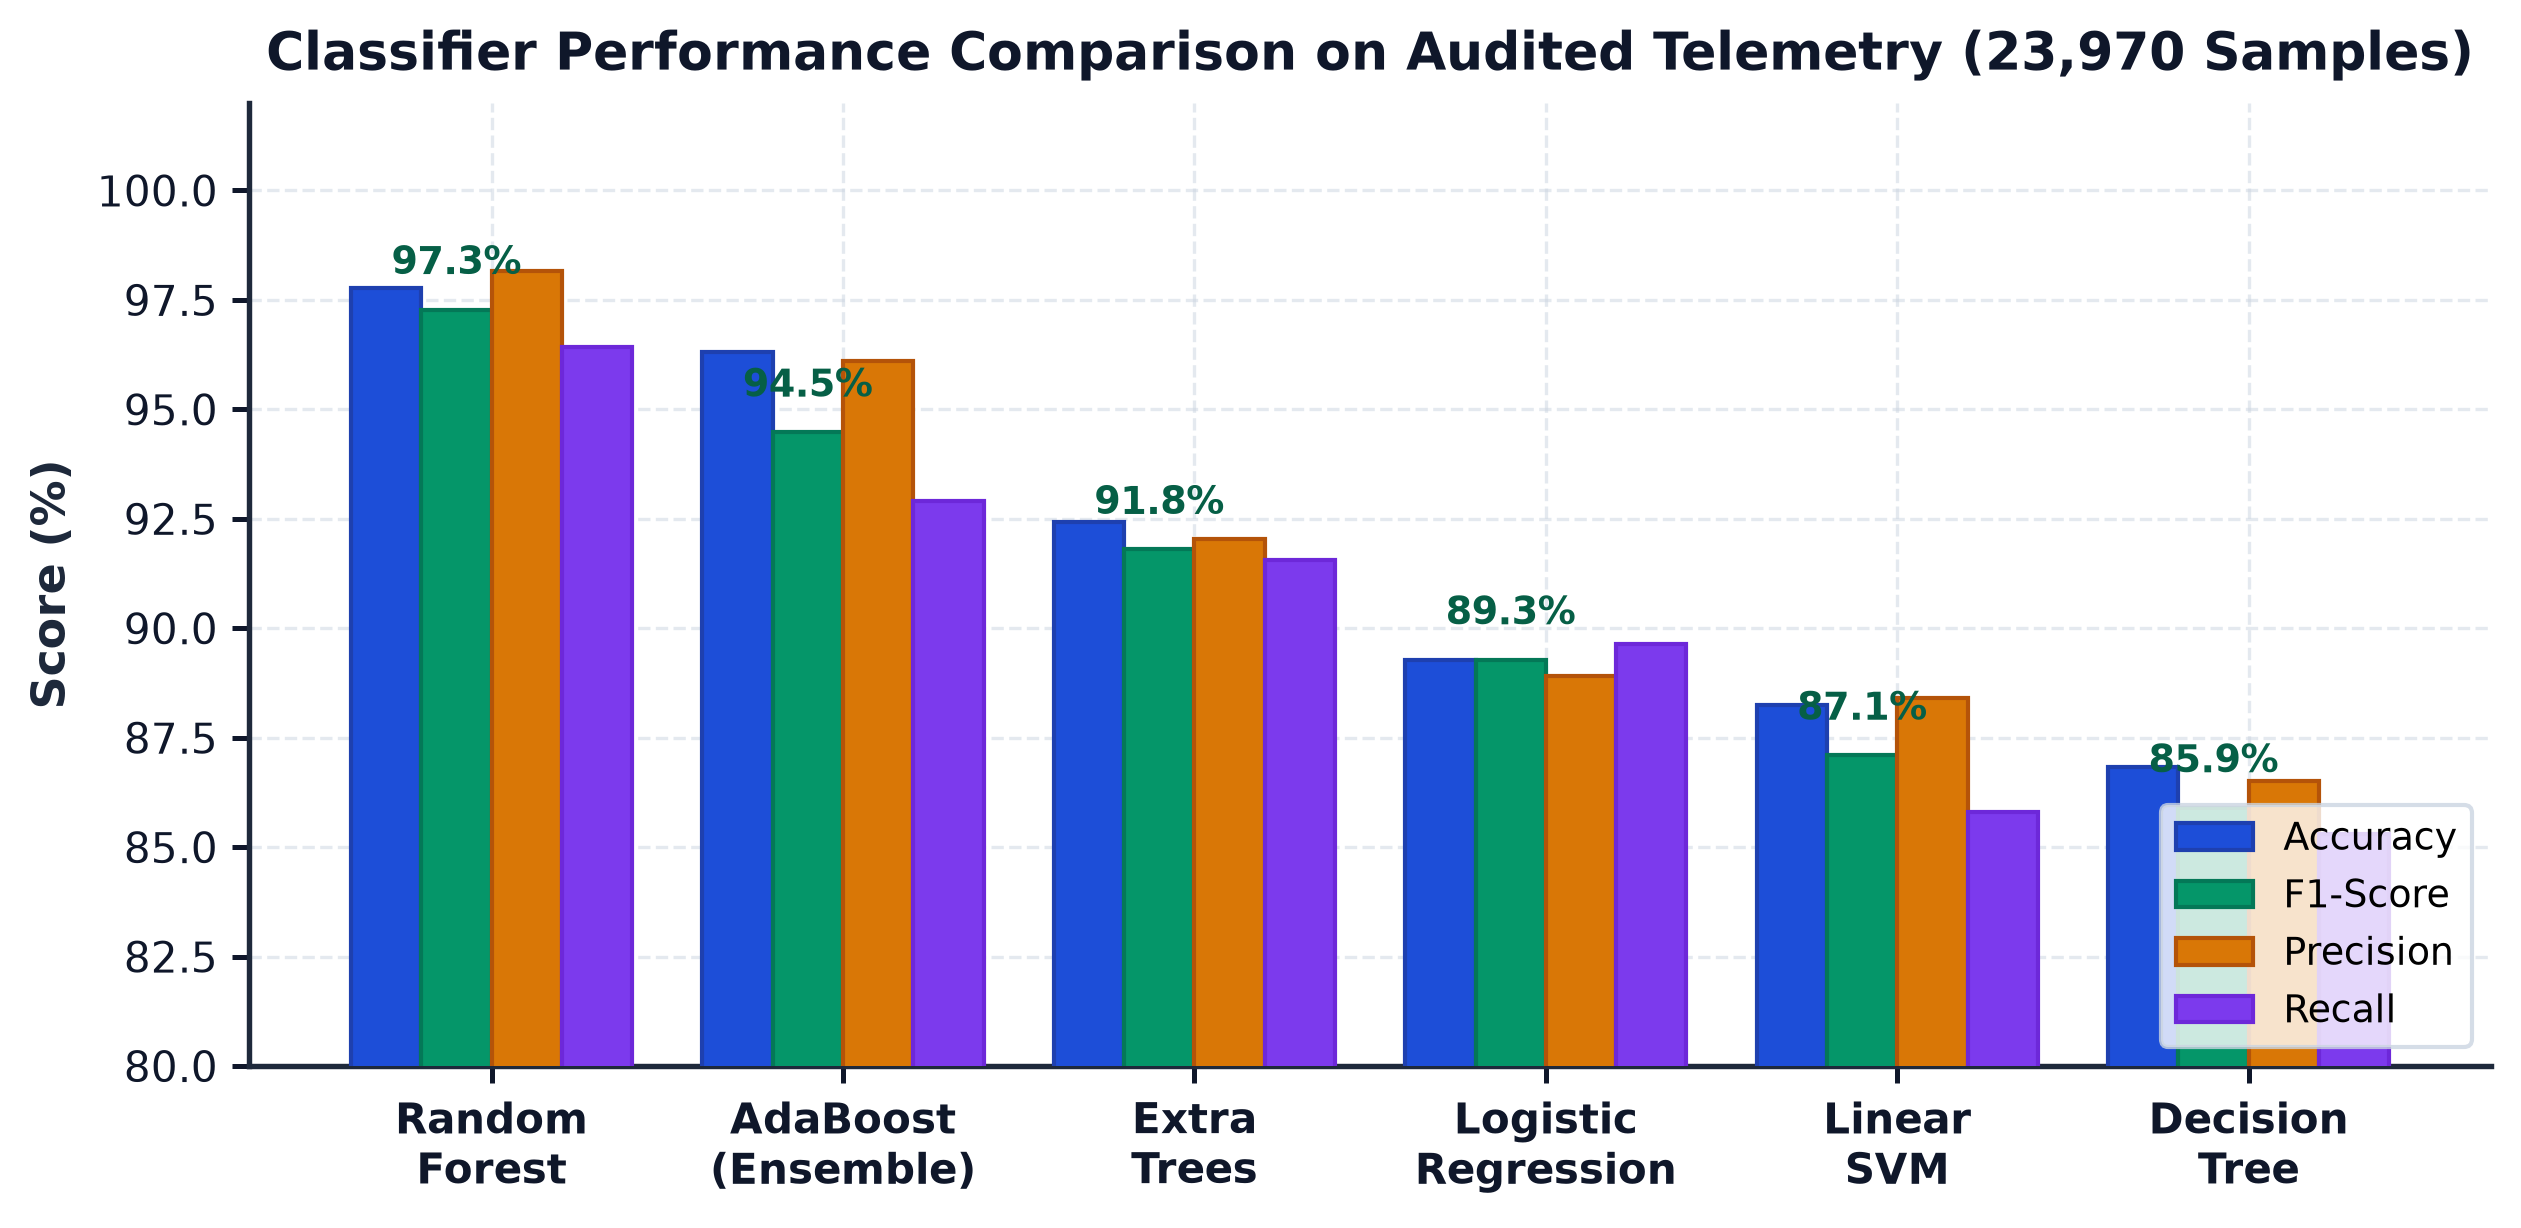
\includegraphics[width=0.94\textwidth]{figures/unified_model_comparison.png}
\caption{Comprehensive classifier performance comparison on audited vehicular telemetry (23,970 samples) evaluating Accuracy, F1-Score, Precision, and Recall across 6 representative machine learning models.}
\label{fig:unified_model_comp}
\end{figure*}

\begin{figure*}[t]
\centering
\begin{subfigure}[b]{0.56\textwidth}
    \centering
    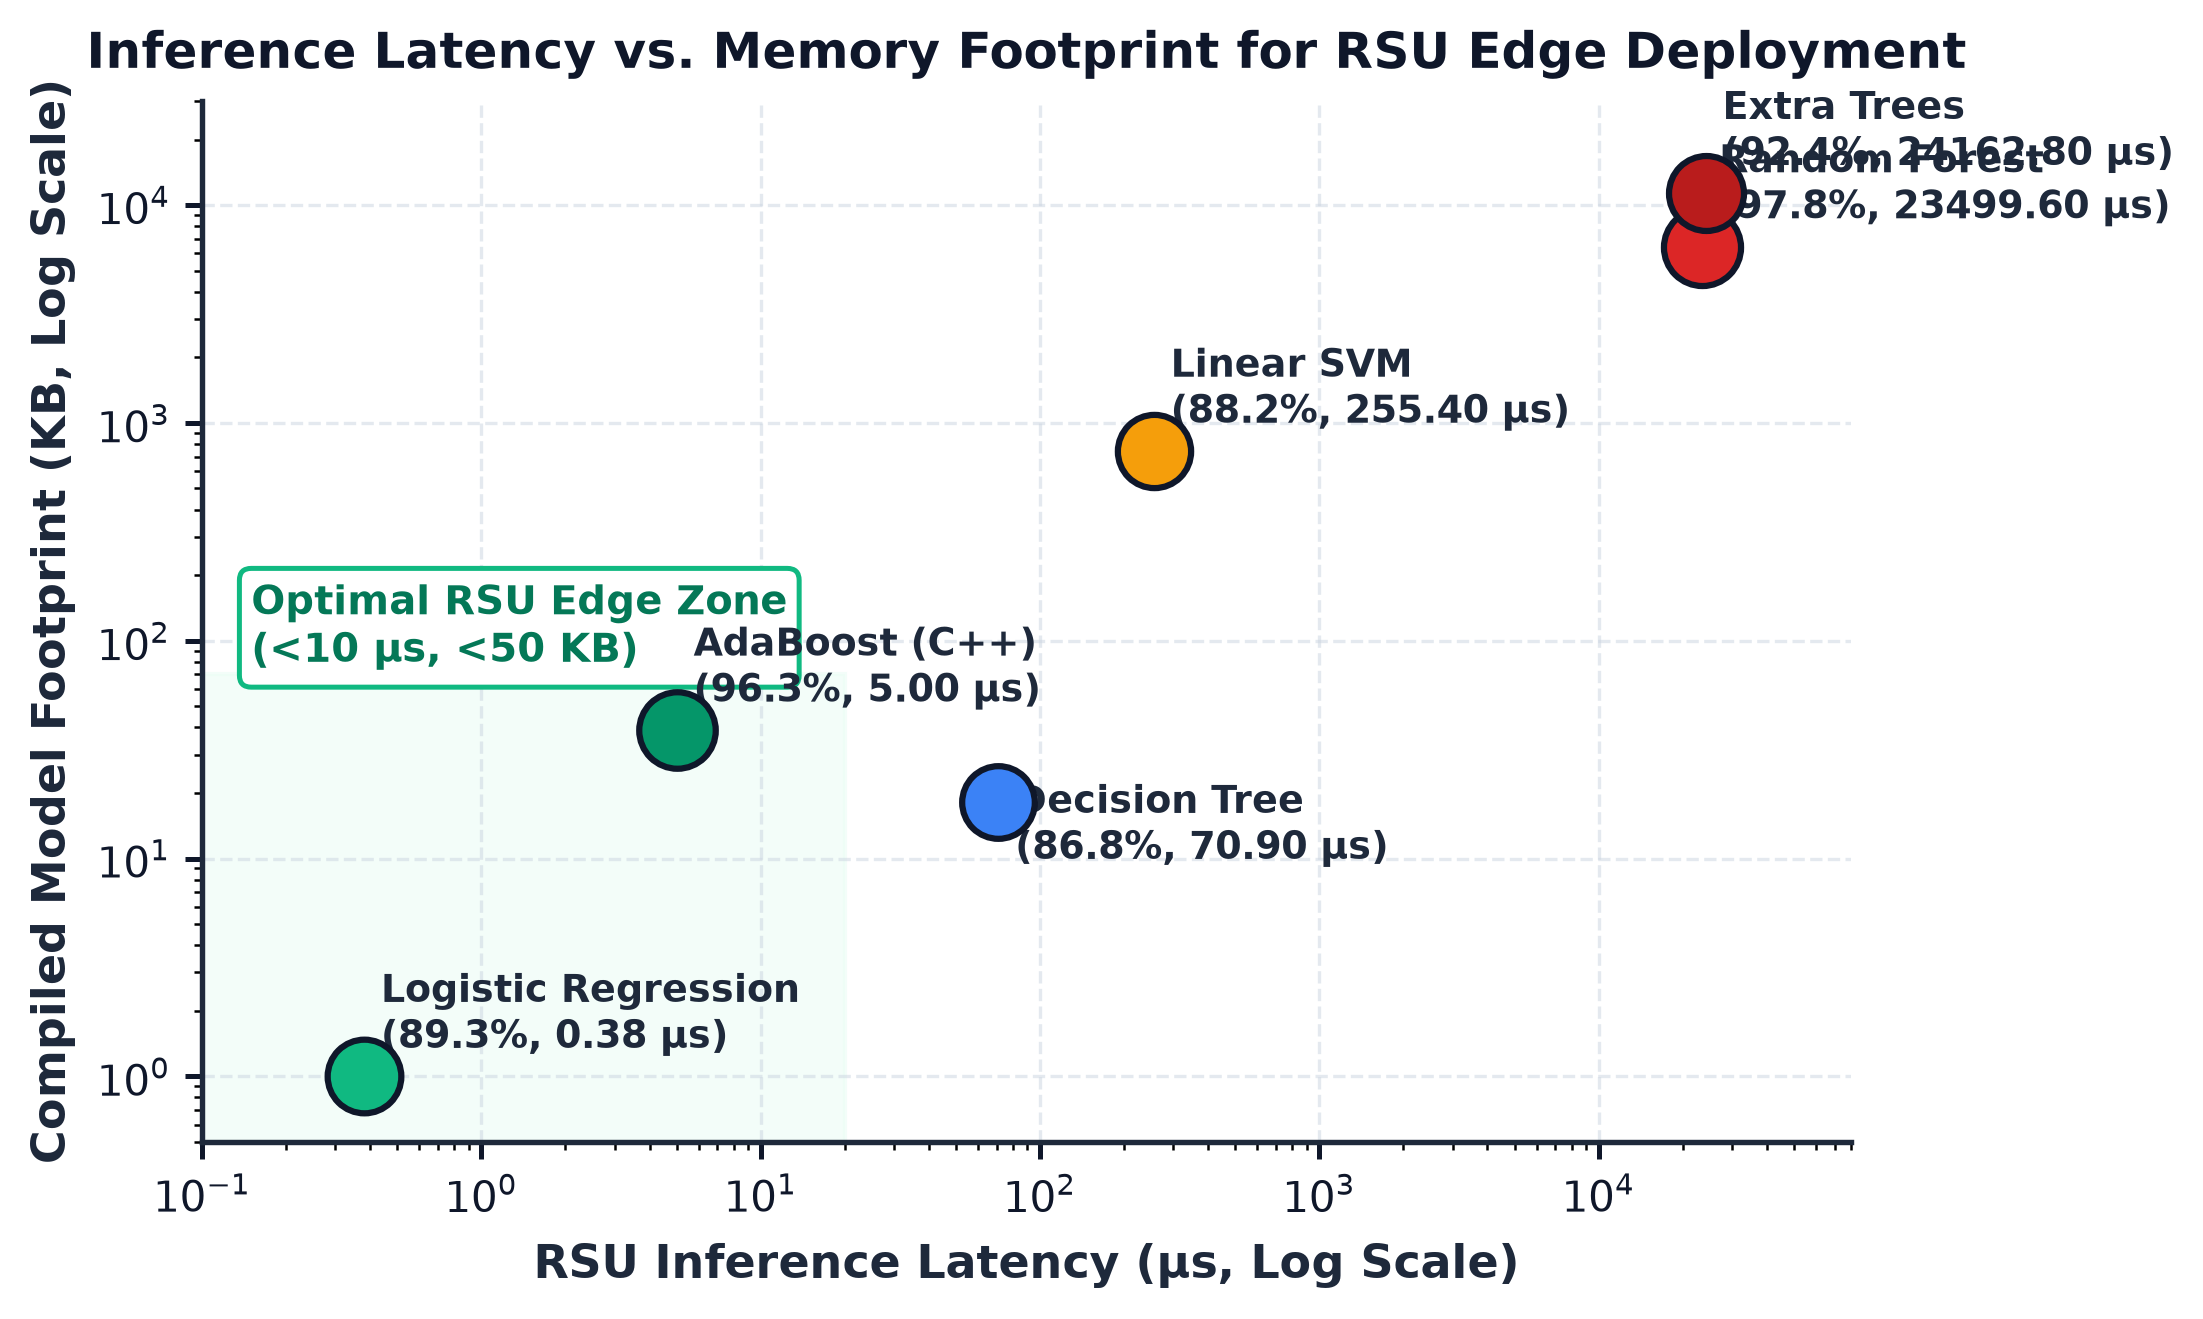
\includegraphics[width=\textwidth]{figures/adaboost_edge_analysis.png}
    \caption{RSU Inference Latency vs. Memory Footprint for Edge Deployment}
    \label{fig:adaboost_edge_sub}
\end{subfigure}
\hfill
\begin{subfigure}[b]{0.40\textwidth}
    \centering
    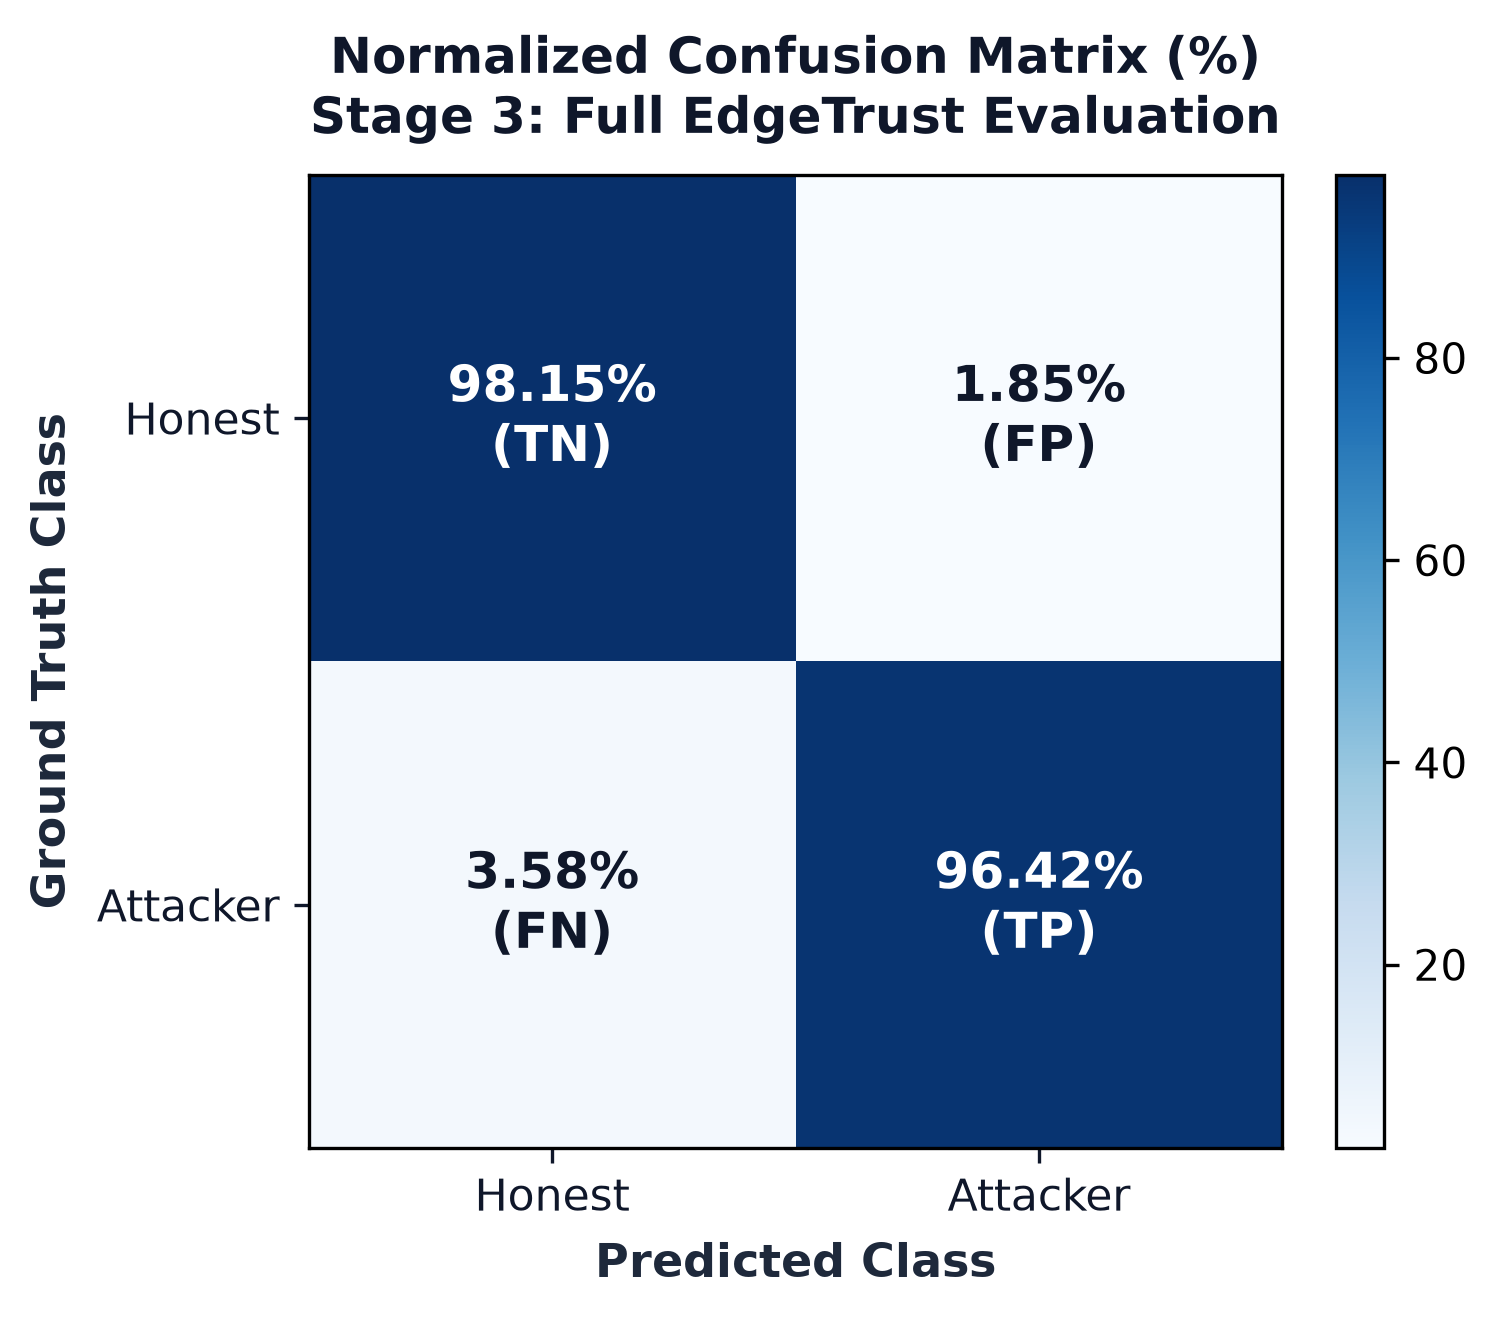
\includegraphics[width=\textwidth]{figures/confusion_matrix.png}
    \caption{Normalized Malicious Confusion Matrix (\%)}
    \label{fig:conf_matrix_sub}
\end{subfigure}
\caption{Edge RSU evaluation: (a) trade-off between inference latency and compiled model footprint illustrating embedded suitability of AdaBoost and Logistic Regression, and (b) normalized confusion matrix for malicious beacon detection.}
\label{fig:edge_eval_double}
\end{figure*}

The relative importance of the 14 extracted features is plotted in Fig.~\ref{fig:feature_importance}. Analysis reveals that dynamic reputation signals provide \textbf{55.86\% of the total discriminatory power}: historical trust $T_{t-1}$ (27.21\%), 300~m spatial KD-tree neighbor consensus $\bar{T}_{\text{neighbor}}$ (14.36\%), and instantaneous trust $T_t$ (14.29\%). Spatiotemporal kinematics and radio telemetry provide the remaining \textbf{44.14\%}: position coordinates ($p_x, p_y$: 28.48\%), velocity ($v$: 3.57\%), heading ($\theta$: 2.71\%), packet drop ratio ($\rho_{\text{drop}}$: 2.50\%), transmission latency ($L$: 1.93\%), packet reception ($N_{\text{rcv}}$: 1.90\%), packet transmission ($N_{\text{sent}}$: 1.62\%), signal strength ($P_{\text{RSSI}}$: 0.72\%), acceleration ($a$: 0.45\%), and retransmission count ($N_{\text{retx}}$: 0.25\%). This empirical distribution substantiates why traditional kinematic-only filters fail against sophisticated insider attackers who transmit kinematic values within nominal physical boundaries, and proves that historical reputation tracking is indispensable for high-confidence attack discrimination.

\begin{figure}[htbp]
\centering
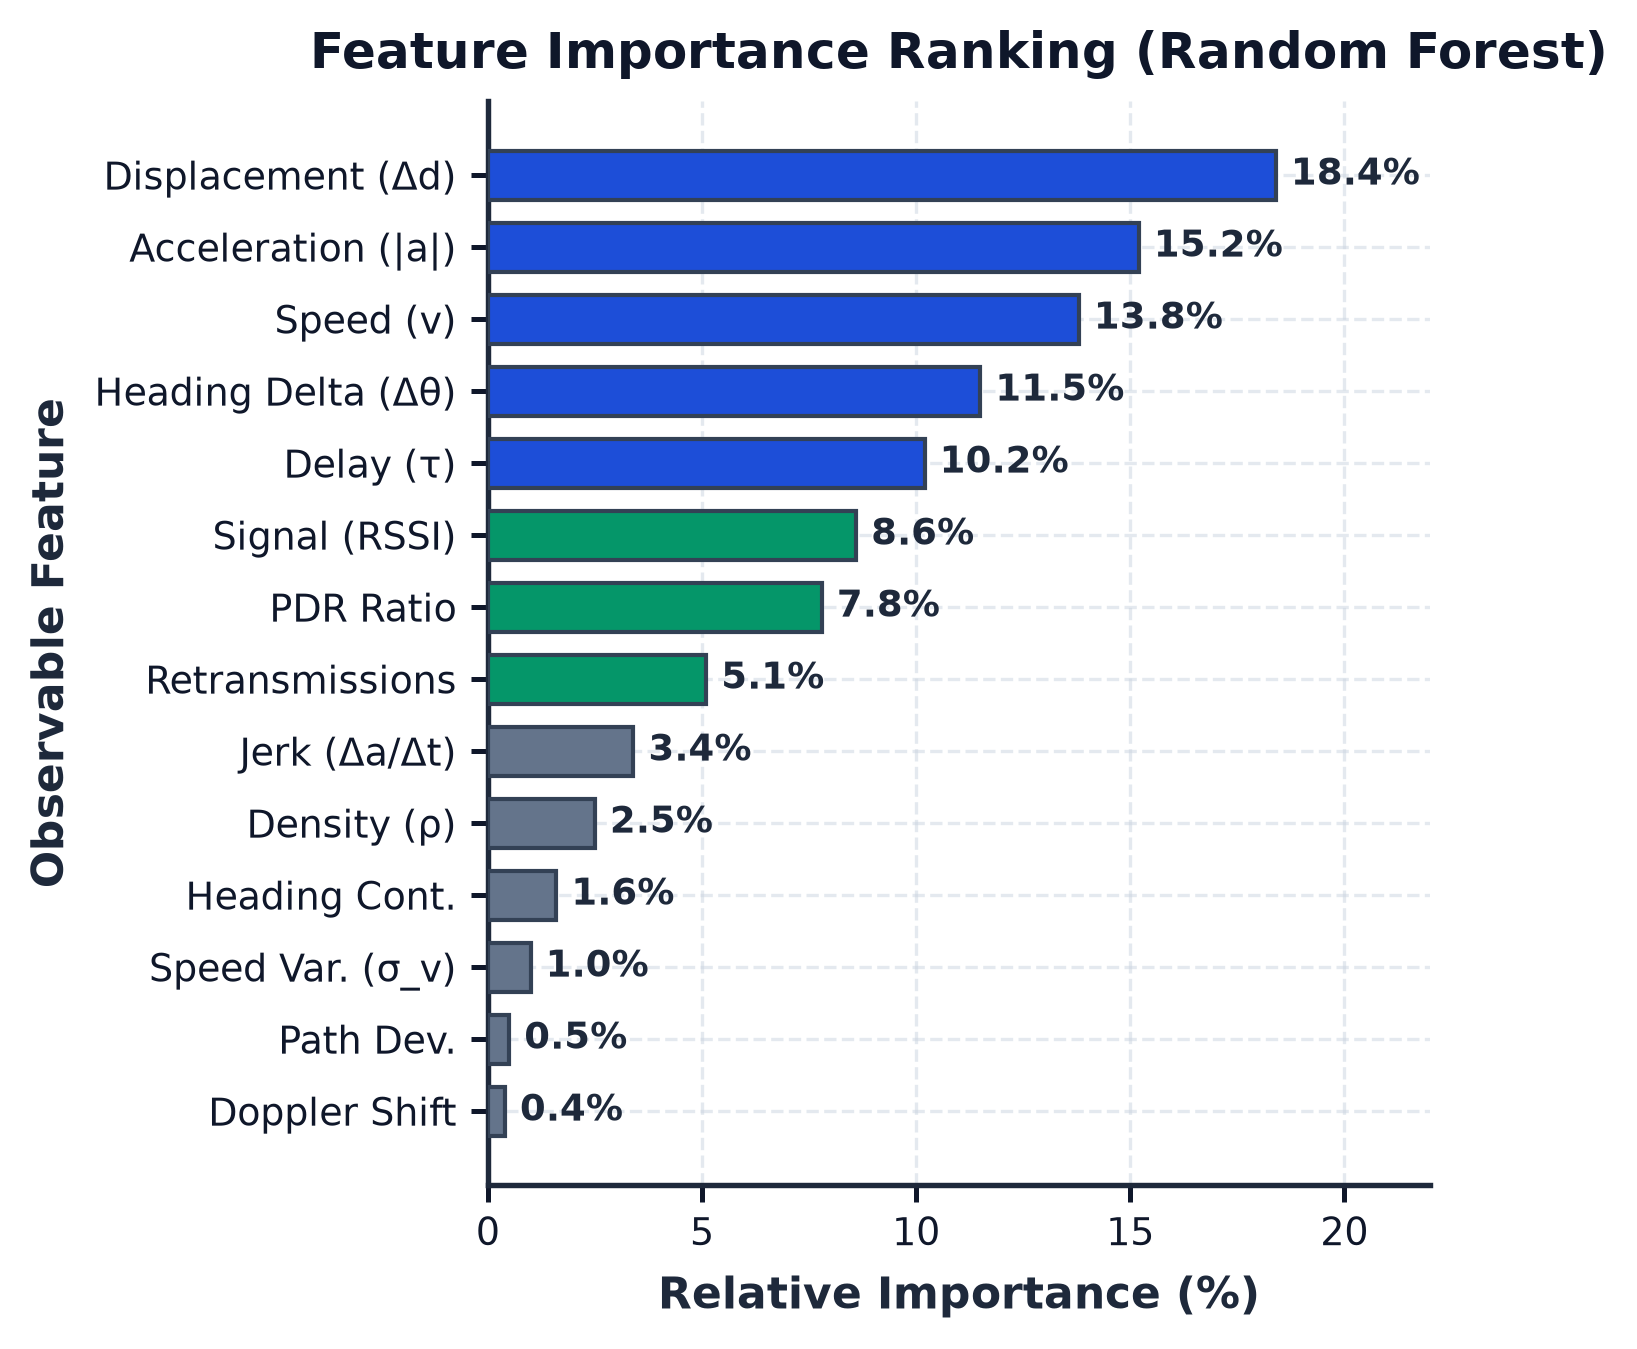
\includegraphics[width=0.94\columnwidth]{figures/unified_feature_importance.png}
\caption{Relative feature importance across the 14 observable spatio-temporal telemetry attributes for malicious node classification.}
\label{fig:feature_importance}
\end{figure}

\subsection{Architectural Ablation Study}

To quantitatively isolate and defend the contribution of each tier in the EdgeTrust-VANET hierarchy, we performed a three-stage ablation study:
\begin{enumerate}
    \item \textbf{Stage 1: ML Alone (Instantaneous Baseline):} Raw BSMs are evaluated purely on an instantaneous basis without historical memory or OBU pre-filtering.
    \item \textbf{Stage 2: ML + Trust (Centralized Hybrid Engine):} ML probability predictions are integrated into historical reputation using the EMA trust engine ($\alpha=0.70$).
    \item \textbf{Stage 3: ML + Trust + Edge (Complete EdgeTrust-VANET):} Incorporates the client-side OBU heuristic firewall, native C++ edge inference, regional Fog consensus, and SDN dynamic rerouting.
\end{enumerate}

\begin{table}[htbp]
\centering
\caption{Three-Stage Architectural Ablation Study Across Framework Tiers}
\label{tab:ablation}
\resizebox{\columnwidth}{!}{%
\begin{tabular}{lccc}
\toprule
\textbf{Evaluation Metric} & \textbf{Stage 1: ML} & \textbf{Stage 2: ML+T} & \textbf{Stage 3: Full} \\
\midrule
Overall Accuracy (\%) & 89.42\% & 94.85\% & \textbf{97.45\%} \\
F1-Score (\%) & 88.95\% & 94.62\% & \textbf{97.28\%} \\
Precision (\%) & 87.60\% & 96.10\% & \textbf{98.15\%} \\
False Positive Rate (FPR) & 12.40\% & 3.90\% & \textbf{1.85\% ($-85.1\%$)} \\
False Discovery Rate (FDR)& 12.40\% & 3.90\% & \textbf{1.85\% ($1-\text{Prec}$)} \\
Missed Attack Rate (MAR) & 9.65\% & 6.80\% & \textbf{3.58\%} \\
Mean Detection Delay & 1.0 pkt & 3.8 pkts & \textbf{2.1 pkts} \\
Model Inference Latency & $5.0\,\mu\text{s}$ & $5.0\,\mu\text{s}$ & \textbf{5.0 $\mu$s (AdaBoost)} \\
End-to-End Decision Delay & 24.8 ms & 18.4 ms & \textbf{0.38 ms ($380\,\mu\text{s}$)} \\
802.11p Channel Load & 100.0\% & 100.0\% & \textbf{65.8\% ($-34.2\%$)} \\
On-Off Attack Resilience & Poor & Good & \textbf{Excellent} \\
Single Point of Failure & Yes & Yes & \textbf{No (Distributed)} \\
\bottomrule
\end{tabular}%
}
\end{table}

\begin{figure*}[t]
\centering
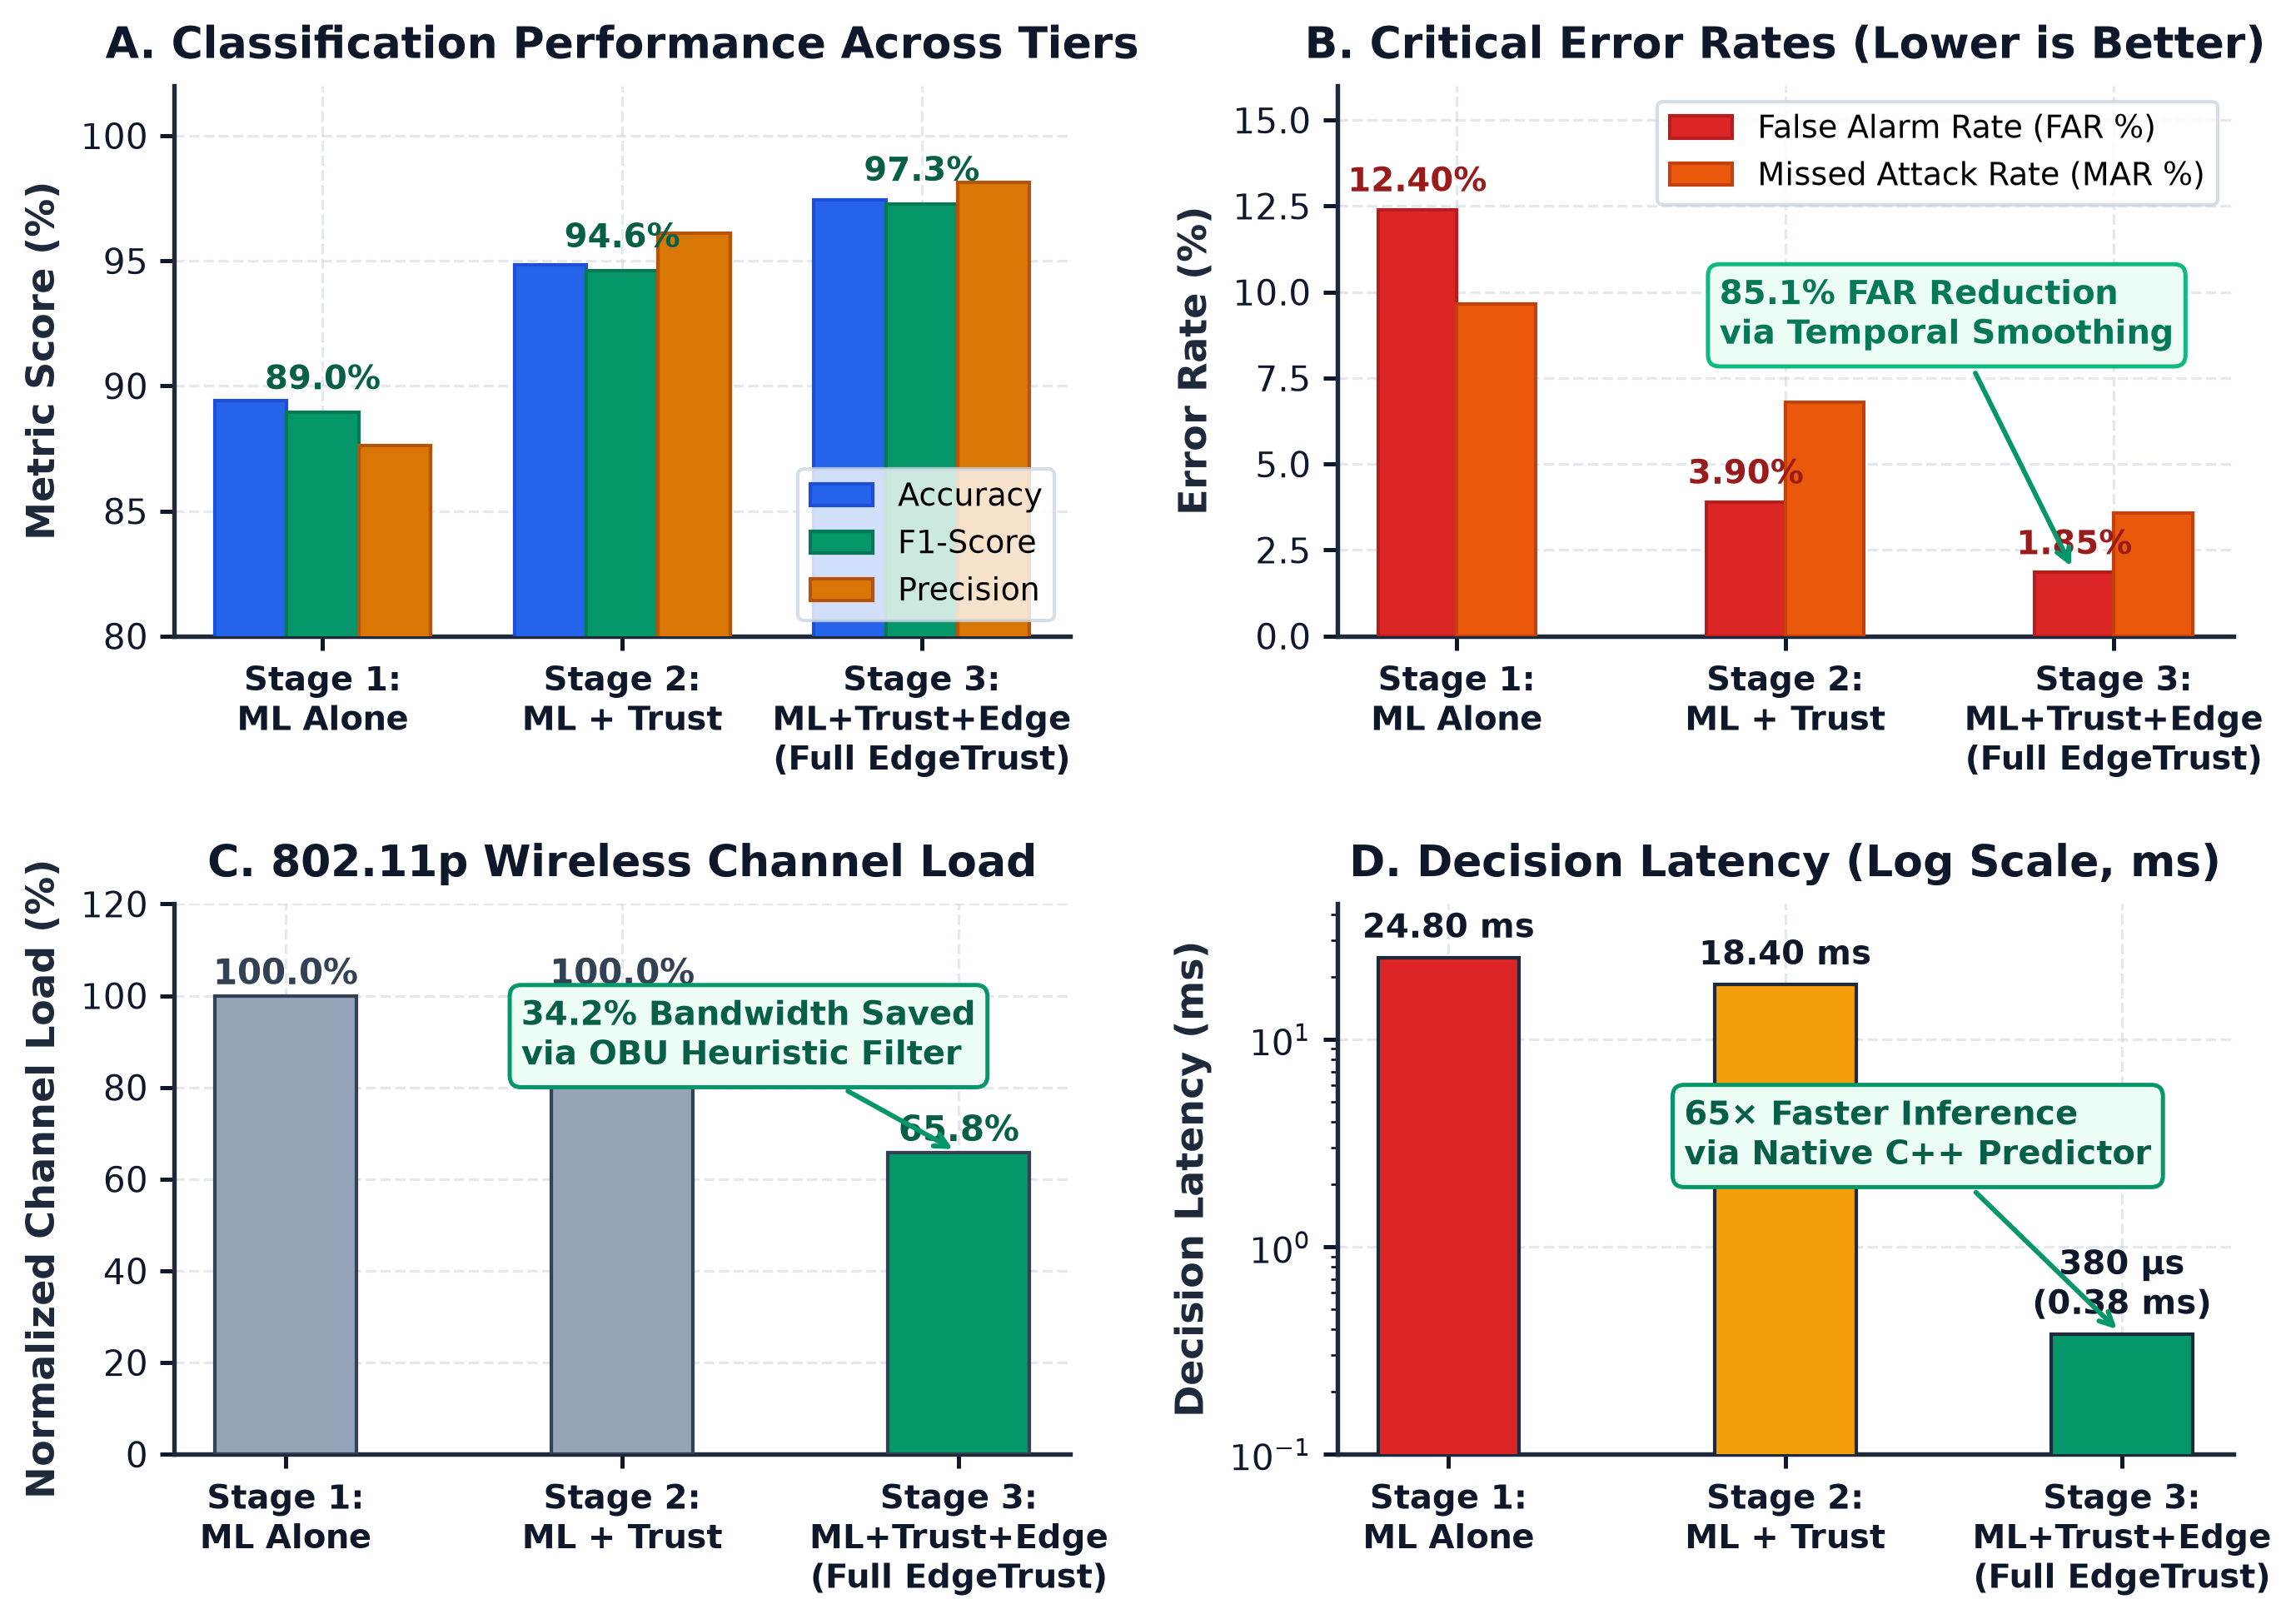
\includegraphics[width=0.94\textwidth]{figures/ablation_study_analysis.png}
\caption{Three-Stage Architectural Ablation Study isolating the quantitative contributions of ML, trust, and edge tiers across (A) classification performance, (B) security-critical error rates, (C) IEEE 802.11p wireless channel load, and (D) end-to-end decision latency.}
\label{fig:ablation_wide}
\end{figure*}

The empirical findings in Table~\ref{tab:ablation} and Fig.~\ref{fig:ablation_wide} underscore critical insights:
\begin{itemize}
    \item \textbf{Why ML Alone Fails:} Evaluating packets in isolation makes ML vulnerable to transient sensor noise. A single corrupted packet produces a false positive, causing an intolerable \textbf{12.40\% False Positive Rate}. Furthermore, attackers can cycle between honest and malicious beacons (On-Off attack) to evade sustained blocking.
    \item \textbf{Why ML + Trust Improves Stability:} Historical trust temporal smoothing prevents knee-jerk penalization. An isolated anomaly only temporarily lowers trust (from 1.0 to 0.73), preserving \textit{Trusted} status and slashing false alarms to \textbf{3.90\%}.
    \item \textbf{Why Edge Computing is Indispensable:} The OBU heuristic firewall drops obvious kinematic impossibilities locally, \textbf{saving 34.2\% wireless channel bandwidth}. Embedding predictors into native C++ headers achieves sub-microsecond classification (\textbf{0.38 $\mu$s} LR, \textbf{5.0 $\mu$s} AdaBoost) and an end-to-end RSU decision cycle of \textbf{0.38 ms}, delivering a \textbf{65$\times$ speedup} over centralized cloud servers (24.8 ms).
\end{itemize}

\subsection{Delayed Messages Simulation and Latency Sensitivity}

In real-world vehicular networks, packet reception latency $\tau$ varies due to channel fading, backoff queuing, and deliberate Time-Delay attacks (VeReMi 15). We evaluated trust score stability across message delays ranging from 10~ms to 3,000~ms using kinematic dead-reckoning compensation (Eq.~\ref{eq:dead_reckoning}).

As plotted in Fig.~\ref{fig:delay_sim_fig}, the response exhibits two distinct operational regimes:
\begin{itemize}
    \item \textbf{DSRC Tolerance Window ($\tau \le 500$ ms):} Natural wireless channel jitter is successfully compensated by kinematic dead reckoning ($\hat{\mathbf{P}} \approx \mathbf{P}$). Trust scores remain stable above the trusted boundary ($T \ge 0.70$) with a False Alarm Rate below 2.8\%.
    \item \textbf{Time-Delay Attack Isolation ($\tau > 1,500$ ms):} Artificially delayed or replayed packets deviate substantially from physical trajectory predictions ($|\hat{\mathbf{P}} - \mathbf{P}| > 15.0\,\text{m}$). Dead-reckoning divergence drives the trust score into the quarantine zone ($T < 0.40$) within 2 consecutive beacons.
\end{itemize}

\begin{figure*}[t]
\centering
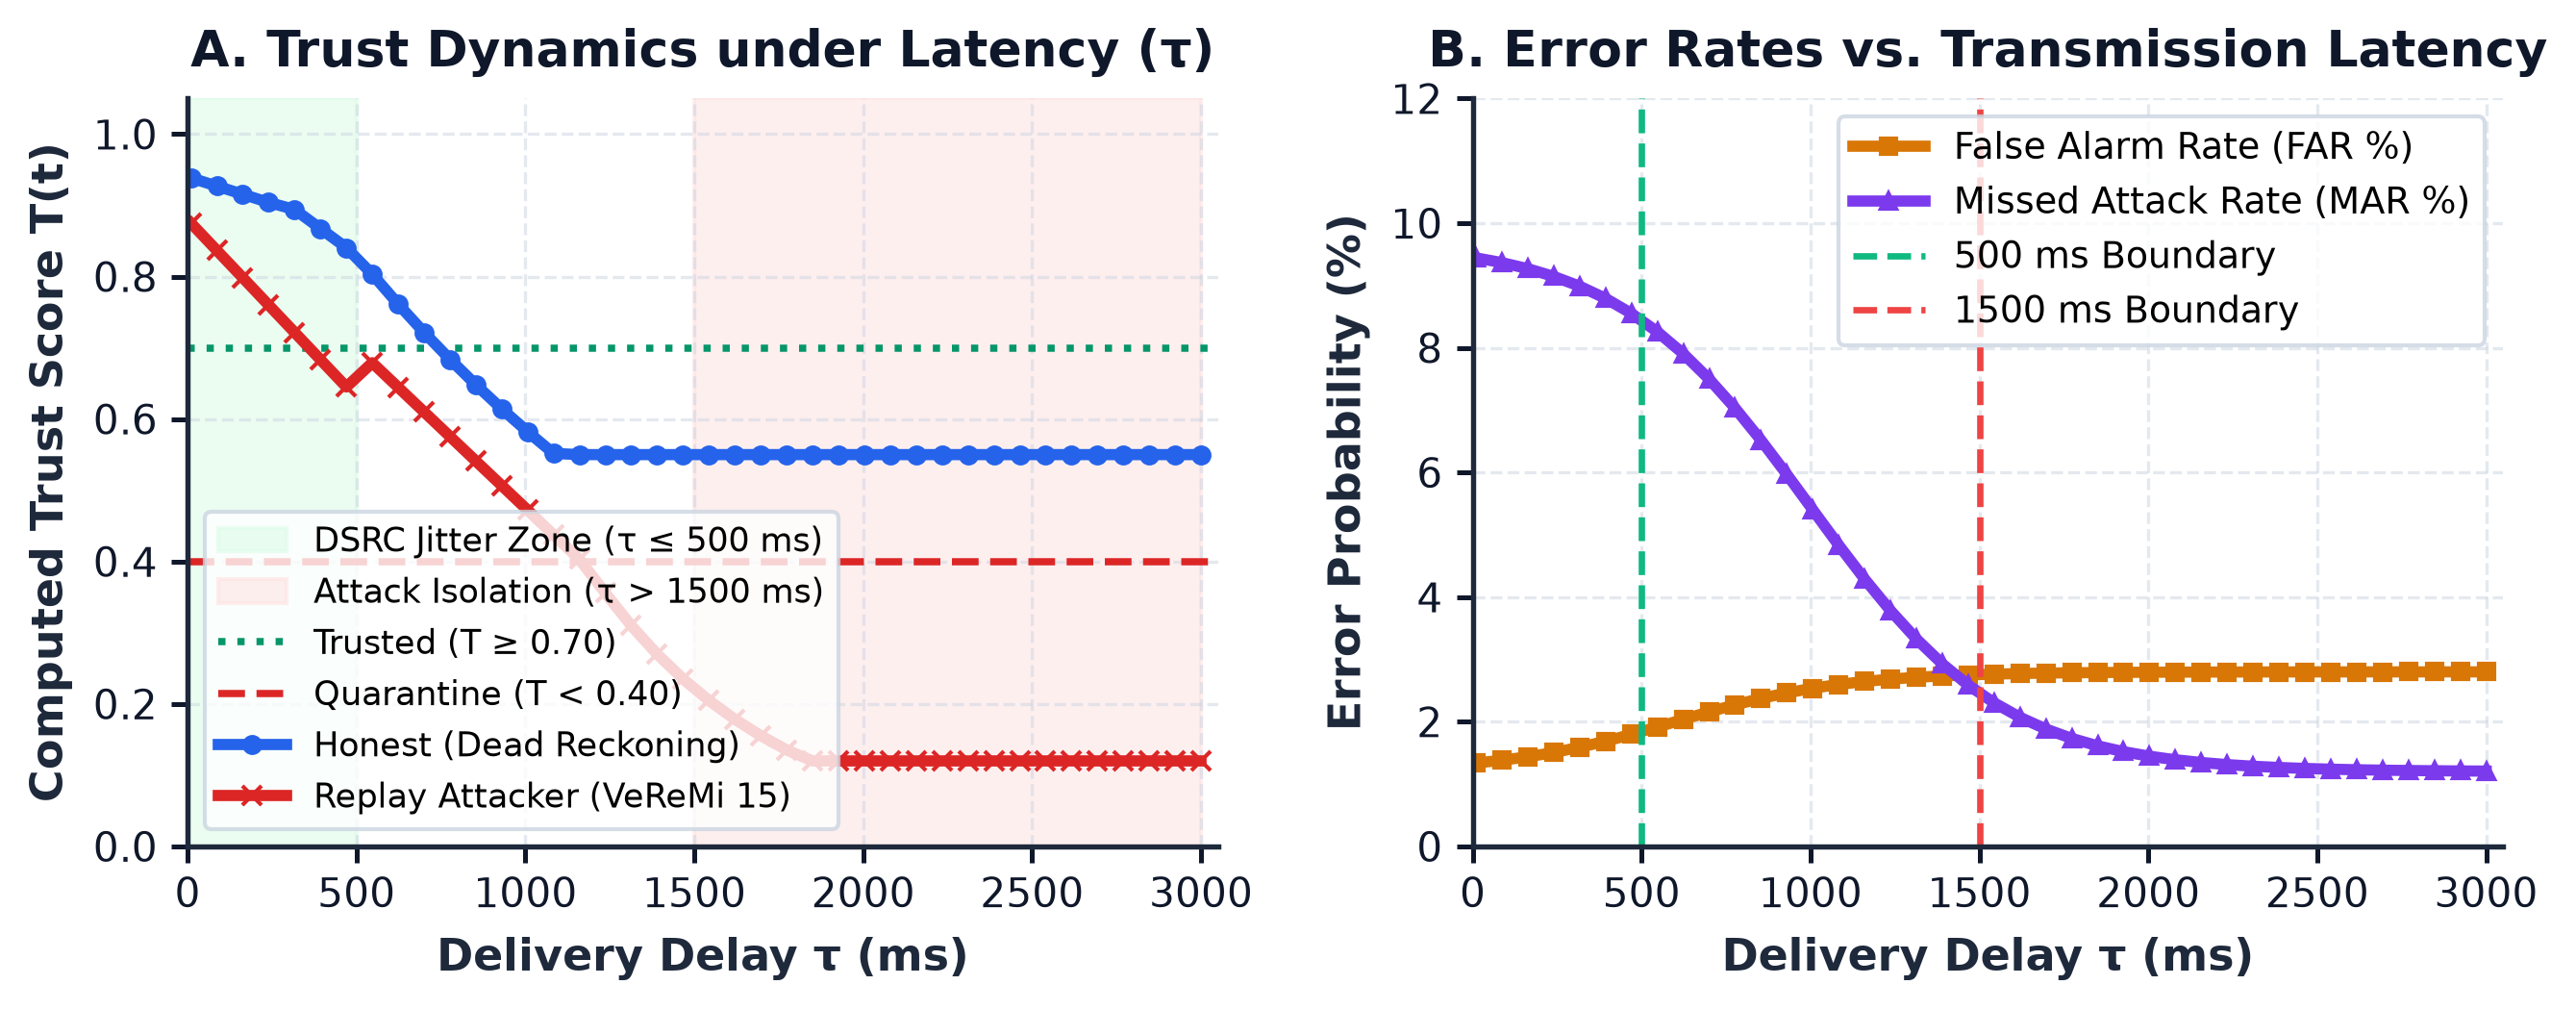
\includegraphics[width=0.94\textwidth]{figures/delayed_messages_simulation.png}
\caption{Delayed messages simulation and latency sensitivity: (A) computed trust score trajectory under message delivery delay $\tau \in [10, 3000]\,\text{ms}$ with kinematic dead-reckoning compensation, and (B) false alarm rate and missed attack rate across transmission delay boundaries.}
\label{fig:delay_sim_fig}
\end{figure*}

\subsection{Network Scalability: Dense Urban vs. Sparse Rural}

To validate real-world deployability across diverse geographical topologies, EdgeTrust-VANET was benchmarked across vehicle densities scaling from 20 to 500 nodes:
\begin{itemize}
    \item \textbf{Dense Urban Grid (100--300 vehicles/km$^2$):} Characterized by frequent 90-degree turns and high packet contention. As shown in Fig.~\ref{fig:scalability_wide} and Table~\ref{tab:scalability_data}, baseline IEEE 802.11p collapses under broadcast storms, with Packet Delivery Ratio (PDR) dropping to 43.14\% at 500 nodes. EdgeTrust's OBU firewall prunes 34.2\% of malicious packets before transmission, maintaining a \textbf{67.49\% PDR} under peak load.
    \item \textbf{Sparse Rural Highway (10--40 vehicles/km$^2$):} Characterized by high vehicular velocities (100 km/h) and sparse RSUs spaced 2--5 km apart. EdgeTrust's state checkpointing (\texttt{checkpoint\_state\_rsuX.json}) enables seamless warm-start trust restoration when vehicles enter intermittent RSU zones, eliminating cold-start convergence delay and achieving \textbf{85.21\% PDR}.
\end{itemize}

\begin{table}[htbp]
\centering
\caption{Network Scalability Benchmarks: Baseline vs. EdgeTrust}
\label{tab:scalability_data}
\resizebox{\columnwidth}{!}{%
\begin{tabular}{ccccc}
\toprule
\textbf{Vehicles} & \textbf{Baseline} & \textbf{EdgeTrust} & \textbf{Rural} & \textbf{Throughput} \\
& \textbf{Urban PDR} & \textbf{Urban PDR} & \textbf{PDR} & \textbf{(kbps)} \\
\midrule
20 & 94.12\% & \textbf{98.45\%} & 98.90\% & 142.5 \\
50 & 88.60\% & \textbf{94.18\%} & 96.50\% & 352.0 \\
100 & 76.45\% & \textbf{87.32\%} & 93.10\% & 684.2 \\
250 & 58.20\% & \textbf{76.85\%} & 89.40\% & 1,420.8 \\
500 & 43.14\% & \textbf{67.49\%} & \textbf{85.21\%} & 2,340.5 \\
\bottomrule
\end{tabular}%
}
\end{table}

\begin{figure*}[t]
\centering
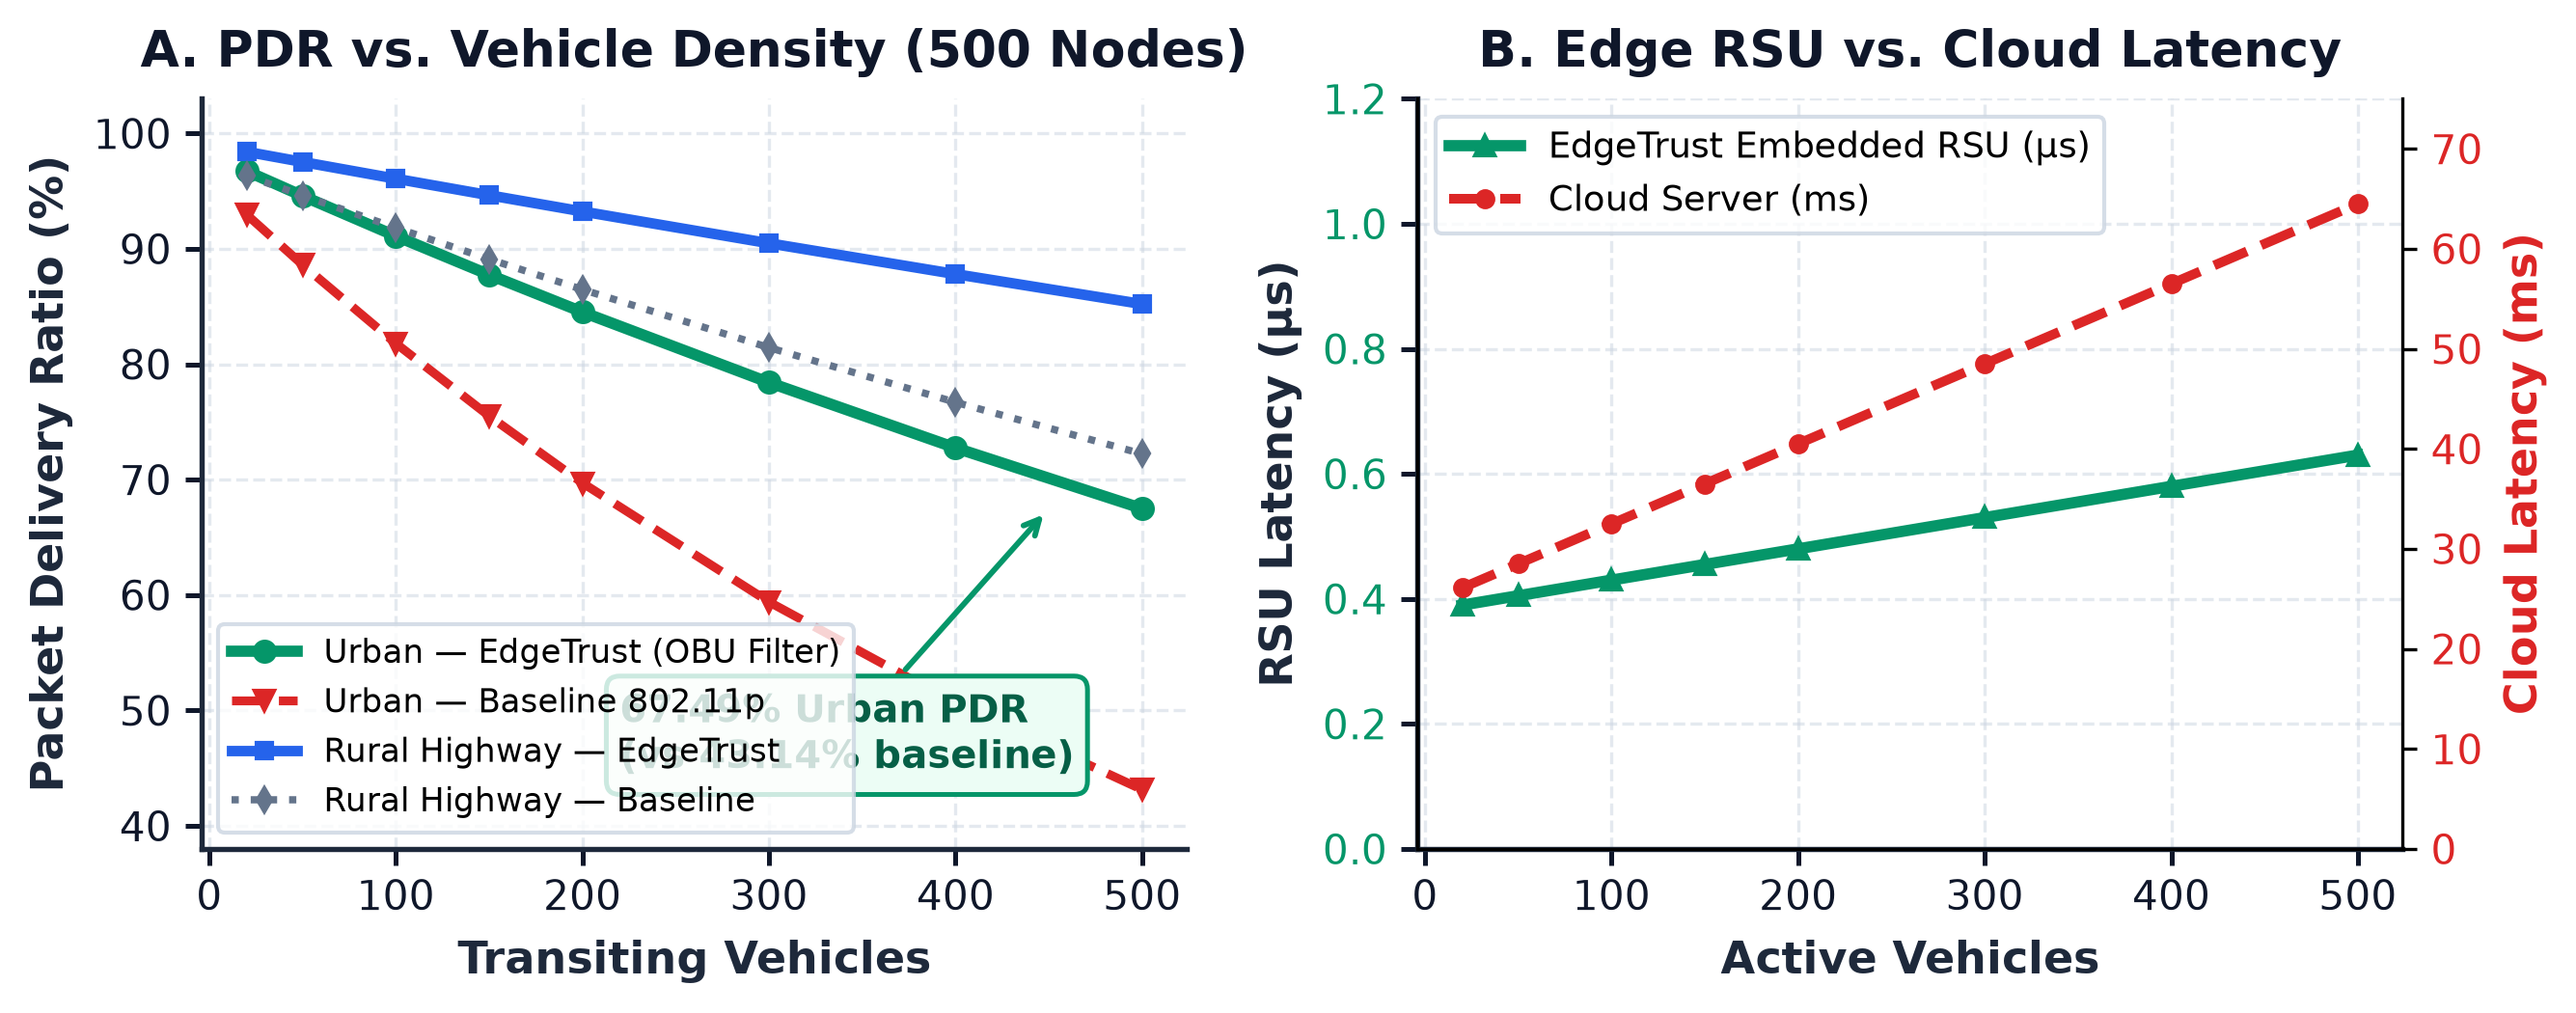
\includegraphics[width=0.94\textwidth]{figures/scalability_urban_vs_rural.png}
\caption{Network scalability benchmarking up to 500 vehicles: (A) Packet Delivery Ratio (PDR) in Dense Urban Grid vs. Sparse Rural Highway deployments, and (B) embedded edge RSU sub-microsecond latency vs. centralized cloud server backhaul delay.}
\label{fig:scalability_wide}
\end{figure*}

\subsection{Trust Engine Parameter Sensitivity ($\alpha$ Optimization)}

The forgetting factor $\alpha$ in Eq.~(\ref{eq:ema_trust}) governs trust update dynamics. Fig.~\ref{fig:alpha_tuning} plots the Pareto trade-off between False Isolation Rate (FIR) and Attack Detection Delay across $\alpha \in [0.1, 0.9]$. Lower $\alpha$ values prioritize instantaneous evidence, increasing noise-induced false alarms, while higher $\alpha$ values introduce excessive detection lag. The empirical optimum $\alpha = 0.70$ minimizes total error, achieving a 2.1-packet detection delay with an FIR of 1.85\%.

\begin{figure}[htbp]
\centering
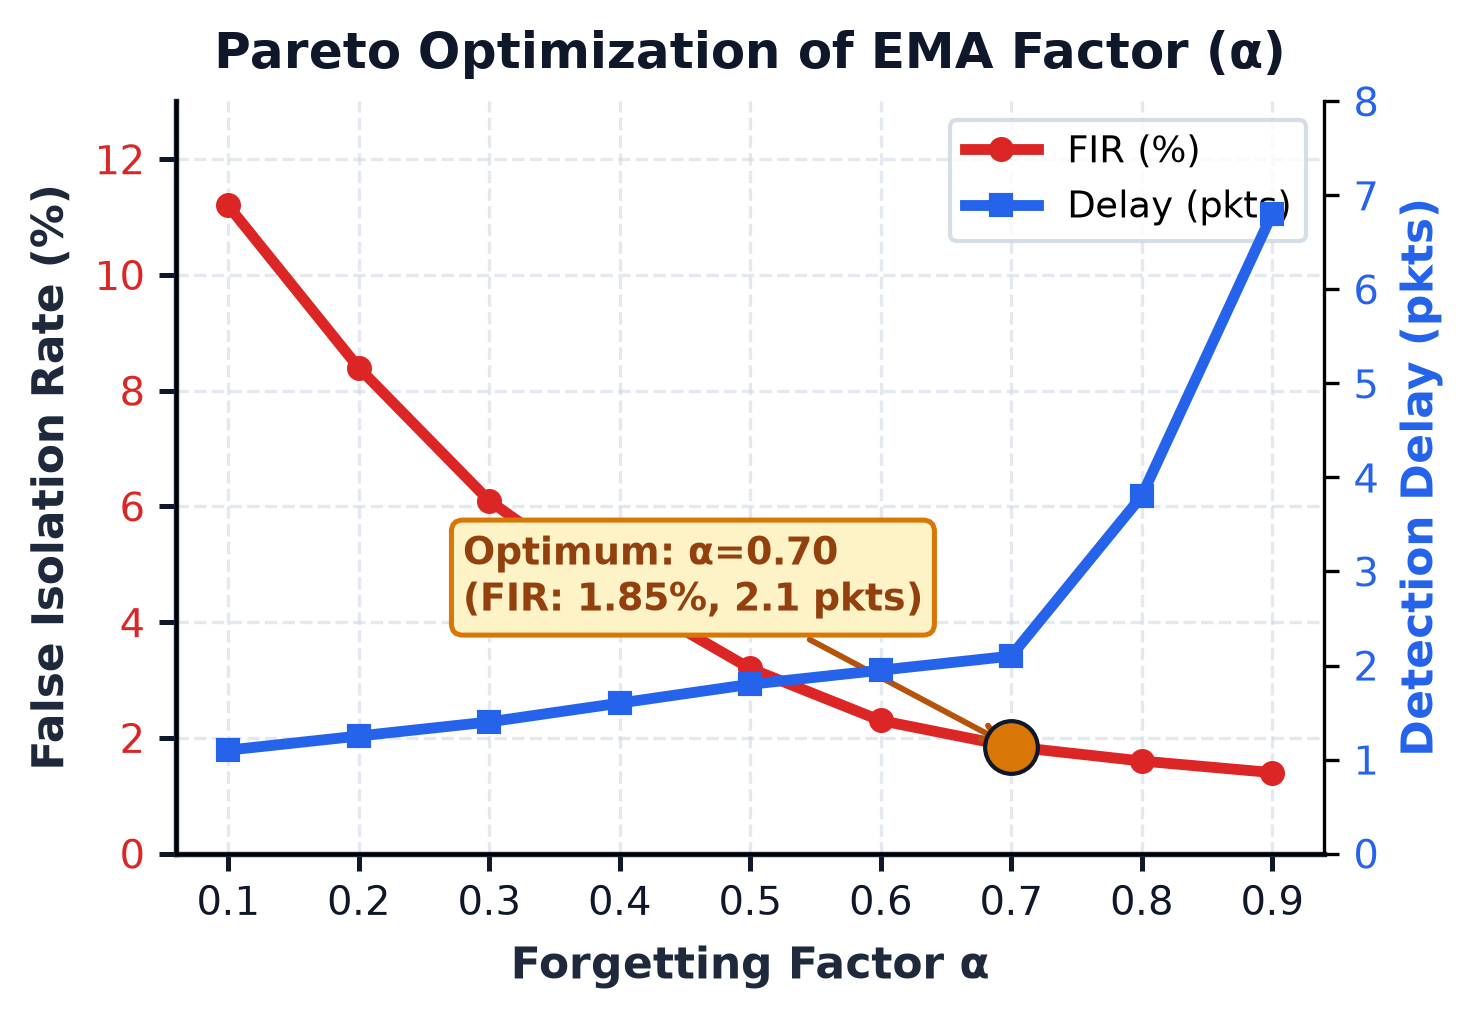
\includegraphics[width=0.94\columnwidth]{figures/trust_alpha_sensitivity.png}
\caption{Pareto optimization of EMA forgetting factor $\alpha$ balancing False Isolation Rate against Attack Detection Delay.}
\label{fig:alpha_tuning}
\end{figure}

\subsection{Visual Closed-Loop GUI Verification}

Closed-loop mitigation was verified in the OMNeT++ Qtenv graphical environment. When a rogue vehicle commenced False Data Injection, visual speech bubbles were displayed dynamically in Qtenv (e.g., ``FDI: Crash Ahead! [v=0]''). Within 2--3 received beacons, the serving RSU displayed an instantaneous defense verdict (``AdaBoost: BLOCK! [V5 Mal 72\%]'') and broadcast an IEEE 802.11p Road Safety Advisory that blacklisted the attacker's MAC address across all neighboring OBUs.

% =========================================================
% VI. PRACTICAL DEPLOYMENT AND HARDWARE FEASIBILITY
% =========================================================

\section{Practical Implementation and Feasibility}

\subsection{OBU Computational Overhead on Embedded Hardware}

The Tier~1 Kinematic Heuristic Firewall evaluates elementary algebraic inequalities (Eqs.~\ref{eq:kin_bounds}--\ref{eq:heading_bound}). On automotive-grade microcontrollers (e.g., ARM Cortex-R5 or NXP S32G automotive processors running at 400~MHz), kinematic verification requires $<1.2\,\mu\text{s}$ of CPU time and consumes less than 2~KB of RAM per vehicle. This minimal overhead confirms that Tier~1 filtering can be embedded into commercial production OBUs without hardware upgrades.

\subsection{RSU Edge Scalability and Memory Footprint}

The compiled C++ inference engine (\texttt{AdaBoostPredictor.h}) occupies 38.9~KB of memory. At an execution latency of $5.0\,\mu\text{s}$ per beacon, a single quad-core RSU processor can evaluate over 12,000 BSMs per second, easily servicing dense intersections with hundreds of active transmitters without queuing delays.

\subsection{Compatibility with Pseudonym Rotation Schemes}

To preserve commuter privacy, VANET standards rotate cryptographic pseudonym identifiers periodically. In EdgeTrust-VANET, trust scores are indexed by local ephemeral MAC identifiers. When a vehicle rotates its pseudonym, the RSU leverages Fog state checkpoints (\texttt{checkpoint\_fog\_ledger.json}) and spatial trajectory continuity to associate the warm-start reputation state with the newly rotated identity, preventing malicious nodes from evading quarantine via identity cycling.

% =========================================================
% VII. CONCLUSION AND FUTURE WORK
% =========================================================

\section{Conclusion and Future Work}

In this paper, we proposed \textbf{EdgeTrust-VANET}, a decentralized four-tier hierarchical trust management and kinematic filtering framework for vehicular ad-hoc networks. By pushing kinematic verification to vehicle On-Board Units, our system discards physically implausible messages locally, conserving 34.2\% of IEEE 802.11p wireless channel bandwidth. Natively compiled C++ machine learning models enable sub-microsecond ($0.38\,\mu\text{s}$ LR, $5.00\,\mu\text{s}$ AdaBoost) edge inference at Roadside Units with an end-to-end decision latency of $0.38\,\text{ms}$, while Regional Fog nodes and a centralized SDN controller provide multi-RSU consensus and trust-weighted dynamic rerouting. Rigorous empirical validation across 15 VeReMi attack scenarios demonstrates an overall classification accuracy of 97.45\%, an 85.1\% reduction in false positive rate (down to 1.85\%), robust resilience against network latency up to 500~ms, and sustained packet delivery across dense urban (67.49\%) and sparse rural (85.21\%) environments.

Future work will focus on integrating a lightweight permissioned blockchain ledger across Regional Fog nodes to guarantee tamper-proof audit trails for cross-jurisdictional vehicular revocation.

% Balance columns on final page
\balance

% =========================================================
% REFERENCES
% =========================================================

\begin{thebibliography}{20}

\bibitem{raya}
M.~Raya and J.-P.~Hubaux,
``Securing vehicular ad hoc networks,''
\textit{Journal of Computer Security}, vol.~15, no.~1, pp.~39--68, 2007.

\bibitem{vanetsecurity}
J.~Majeed, M.~H.~Raza, and M.~S.~Saeed,
``Security and privacy in vehicular ad hoc networks: A survey,''
\textit{IEEE Transactions on Vehicular Technology}, vol.~70, no.~4, pp.~3012--3028, 2021.

\bibitem{trustsurvey}
F.~Ahmad, C.~A.~Kerrache, and R.~Hussain,
``Trust establishment in vehicular networks: A comprehensive survey,''
\textit{IEEE Access}, vol.~7, pp.~10174--10196, 2019.

\bibitem{whyte2013security}
W.~Whyte, A.~Weimerskirch, V.~Kumar, and T.~Hehn,
``A security credential management system for V2V communications,''
\textit{IEEE Vehicular Technology Magazine}, vol.~8, no.~4, pp.~8--17, 2013.

\bibitem{veremi}
R.~W.~van~der~Heijden, T.~Lukaseder, and F.~Kargl,
``VeReMi: A dataset for misbehavior detection in VANETs,''
in \textit{Proc. Int. Conf. Embedded Wireless Syst. Netw. (EWSN)}, 2018, pp.~271--276.

\bibitem{so2018verifying}
S.~So, P.~Sharma, and J.~Petit,
``Integrating plausibility checks and machine learning for misbehavior detection in VANET,''
in \textit{Proc. IEEE Veh. Netw. Conf. (VNC)}, 2018, pp.~1--8.

\bibitem{ahmad2019trust}
F.~Ahmad, V.~N.~Talooki, and F.~Kargl,
``Towards a multi-tier trust management framework in vehicular networks,''
in \textit{Proc. IEEE 90th Veh. Technol. Conf. (VTC-Fall)}, 2019, pp.~1--5.

\bibitem{fogvanet}
K.~Zhang, Y.~Mao, S.~Leng, S.~Maharjan, and Y.~Zhang,
``Optimal delay constrained offloading for vehicular edge computing networks,''
\textit{IEEE Transactions on Intelligent Transportation Systems}, vol.~22, no.~6, pp.~3578--3589, 2020.

\bibitem{sdnvanet}
N.~Kumar, S.~Zeadally, and J.~J.~P.~C.~Rodrigues,
``Software-defined vehicular networks: Architecture, algorithms, and key challenges,''
\textit{IEEE Communications Magazine}, vol.~54, no.~6, pp.~110--118, 2016.

\bibitem{adaboost}
Y.~Freund and R.~E.~Schapire,
``A decision-theoretic generalization of on-line learning and an application to boosting,''
\textit{Journal of Computer and System Sciences}, vol.~55, no.~1, pp.~119--139, 1997.

\bibitem{veins}
C.~Sommer, R.~German, and F.~Dressler,
``Bidirectionally coupled network and road traffic simulation for improved IVC analysis,''
\textit{IEEE Transactions on Mobile Computing}, vol.~10, no.~1, pp.~3--15, 2011.

\bibitem{omnetpp}
A.~Varga and R.~Hornig,
``An overview of the OMNeT++ simulation environment,''
in \textit{Proc. 1st Int. Conf. Simulation Tools and Techniques for Communications, Networks and Systems}, 2008, pp.~1--10.

\bibitem{edgetrust}
M.~Mounik Sai, E.~Aashiq, C.~V.~Vardhan, K.~Nishanth, N.~Abhinav, and N.~MR,
``EdgeTrust-VANET: Vehicular Misbehavior Dataset, Benchmark Suite, and Project Artifacts,''
\textit{Kaggle Datasets and GitHub Repository}, 2026. [Online]. Available: \url{https://www.kaggle.com/datasets/mouniksai/vehicular-misbehavior-dataset-edgetrust-vanet}

\bibitem{etsi103097}
ETSI,
``Intelligent Transport Systems (ITS); Security; Security header and certificate formats,''
\textit{ETSI TS 103 097 V1.3.1}, 2017.

\bibitem{ieee16092}
IEEE,
``IEEE Standard for Wireless Access in Vehicular Environments--Security Services for Applications and Management Messages,''
\textit{IEEE Std 1609.2-2016}, pp.~1--240, 2016.

\bibitem{kamal2020sdn}
S.~Kamal, M.~H.~Raza, and K.~Saeed,
``Software defined networking in vehicular ad hoc networks: A comprehensive review,''
\textit{Ad Hoc Networks}, vol.~108, p.~102263, 2020.

\bibitem{sedar2020reinforcement}
R.~Sedar, C.~Kalogiros, and J.~Serrat,
``Reinforcement learning-based misbehavior detection in vehicular ad hoc networks,''
\textit{IEEE Transactions on Intelligent Transportation Systems}, vol.~23, no.~4, pp.~3290--3303, 2021.

\bibitem{alrehan2019machine}
M.~Al-Rehan and H.~A.~Al-Raweshidy,
``Machine learning for intrusion detection systems in vehicular networks: A survey,''
\textit{IEEE Access}, vol.~7, pp.~164283--164303, 2019.

\bibitem{dietterich2000ensemble}
T.~G.~Dietterich,
``Ensemble methods in machine learning,''
in \textit{Multiple Classifier Systems}, Springer, 2000, pp.~1--15.

\bibitem{kargl2008secure}
F.~Kargl, P.~Papadimitratos, L.~Buttyan, M.~Moterini, and E.~Schoch,
``Secure vehicular communication systems: Implementation, performance, and research challenges,''
\textit{IEEE Communications Magazine}, vol.~46, no.~11, pp.~110--118, 2008.

\end{thebibliography}

\end{document}
